\section{Introduction}

In this chapter I aim to find out whether adding feedback loops to the genetic toggle switch increases its robustness to parameter fluctuations. To do this, I use \acrshort{abc} \acrshort{smc} model selection, which is capable of selecting the most robust model for a given model behaviour.

Structurally this chapter is organised as follows: In the first section I examine the genetic toggle switch with no added feedback loops. I use a parameter scan to find the parameter values that make it bistable and then use \acrshort{abc} \acrshort{smc} for parameter inference for a switch-like behaviour. In the following section I examine the effect that the addition of feedback loops to the genetic toggle switch has on its stability, and select the switch architectures that are capable of bistable behaviour. Finally, I use ABC-SysBio model selection to select the most robust model out of the bistable switches.


%First parameter scan in order to determine the parameter values that can produce the desired behaviour. Then ABC parameter estimation to determine whether the models used are capable of the desired behaviour. Finally, I use ABC-SysBio model selection to select the most robust model. 


\section{The genetic toggle switch}
%the following is copy paste from SF:
\textcite{Gardner:2000vha} constructed the first synthetic genetic toggle switch. Their model consisted of two mutually repressing transcription factors, and is defined by the following \acrshort{ode}s:

\begin{align}\label{eq:gards}
\frac{du}{dt} &= \frac{a_1}{1+v^{\beta}} - u \\
\frac{dv}{dt} &= \frac{a_2}{1+u^{\gamma }} - v,
\end{align}

\noindent where \textit{u} is the concentration of repressor 1, \textit{v} the concentration of repressor 2, $a_1$ and $a_2$ denote the effective rates of synthesis of repressors 1 and 2 respectively, β is the cooperativity of repression of promoter 1 and γ of repressor 2. 

First, I study the model given in Equations~\ref{eq:gards} by conducting a bifurcation analysis using the PyDSTool~\autocite{Clewley:2012kj} in order to determine whether it is capable of bistable behaviour. The system has two stable steady states and one unstable steady state when $a_1$ and $a_2$ are set to 10, and β, γ set to 2, as shown in Figure~\ref{fig:Gard_CS}B. The bifurcation analysis shows that by varying the parameter for the effective rate of synthesis of repressor 1 while all other parameters remain constant, the system is bistable when 5 \ge{} $a_1$ \le{} 31.



\begin{figure*}[htbp]
	\begin{center}
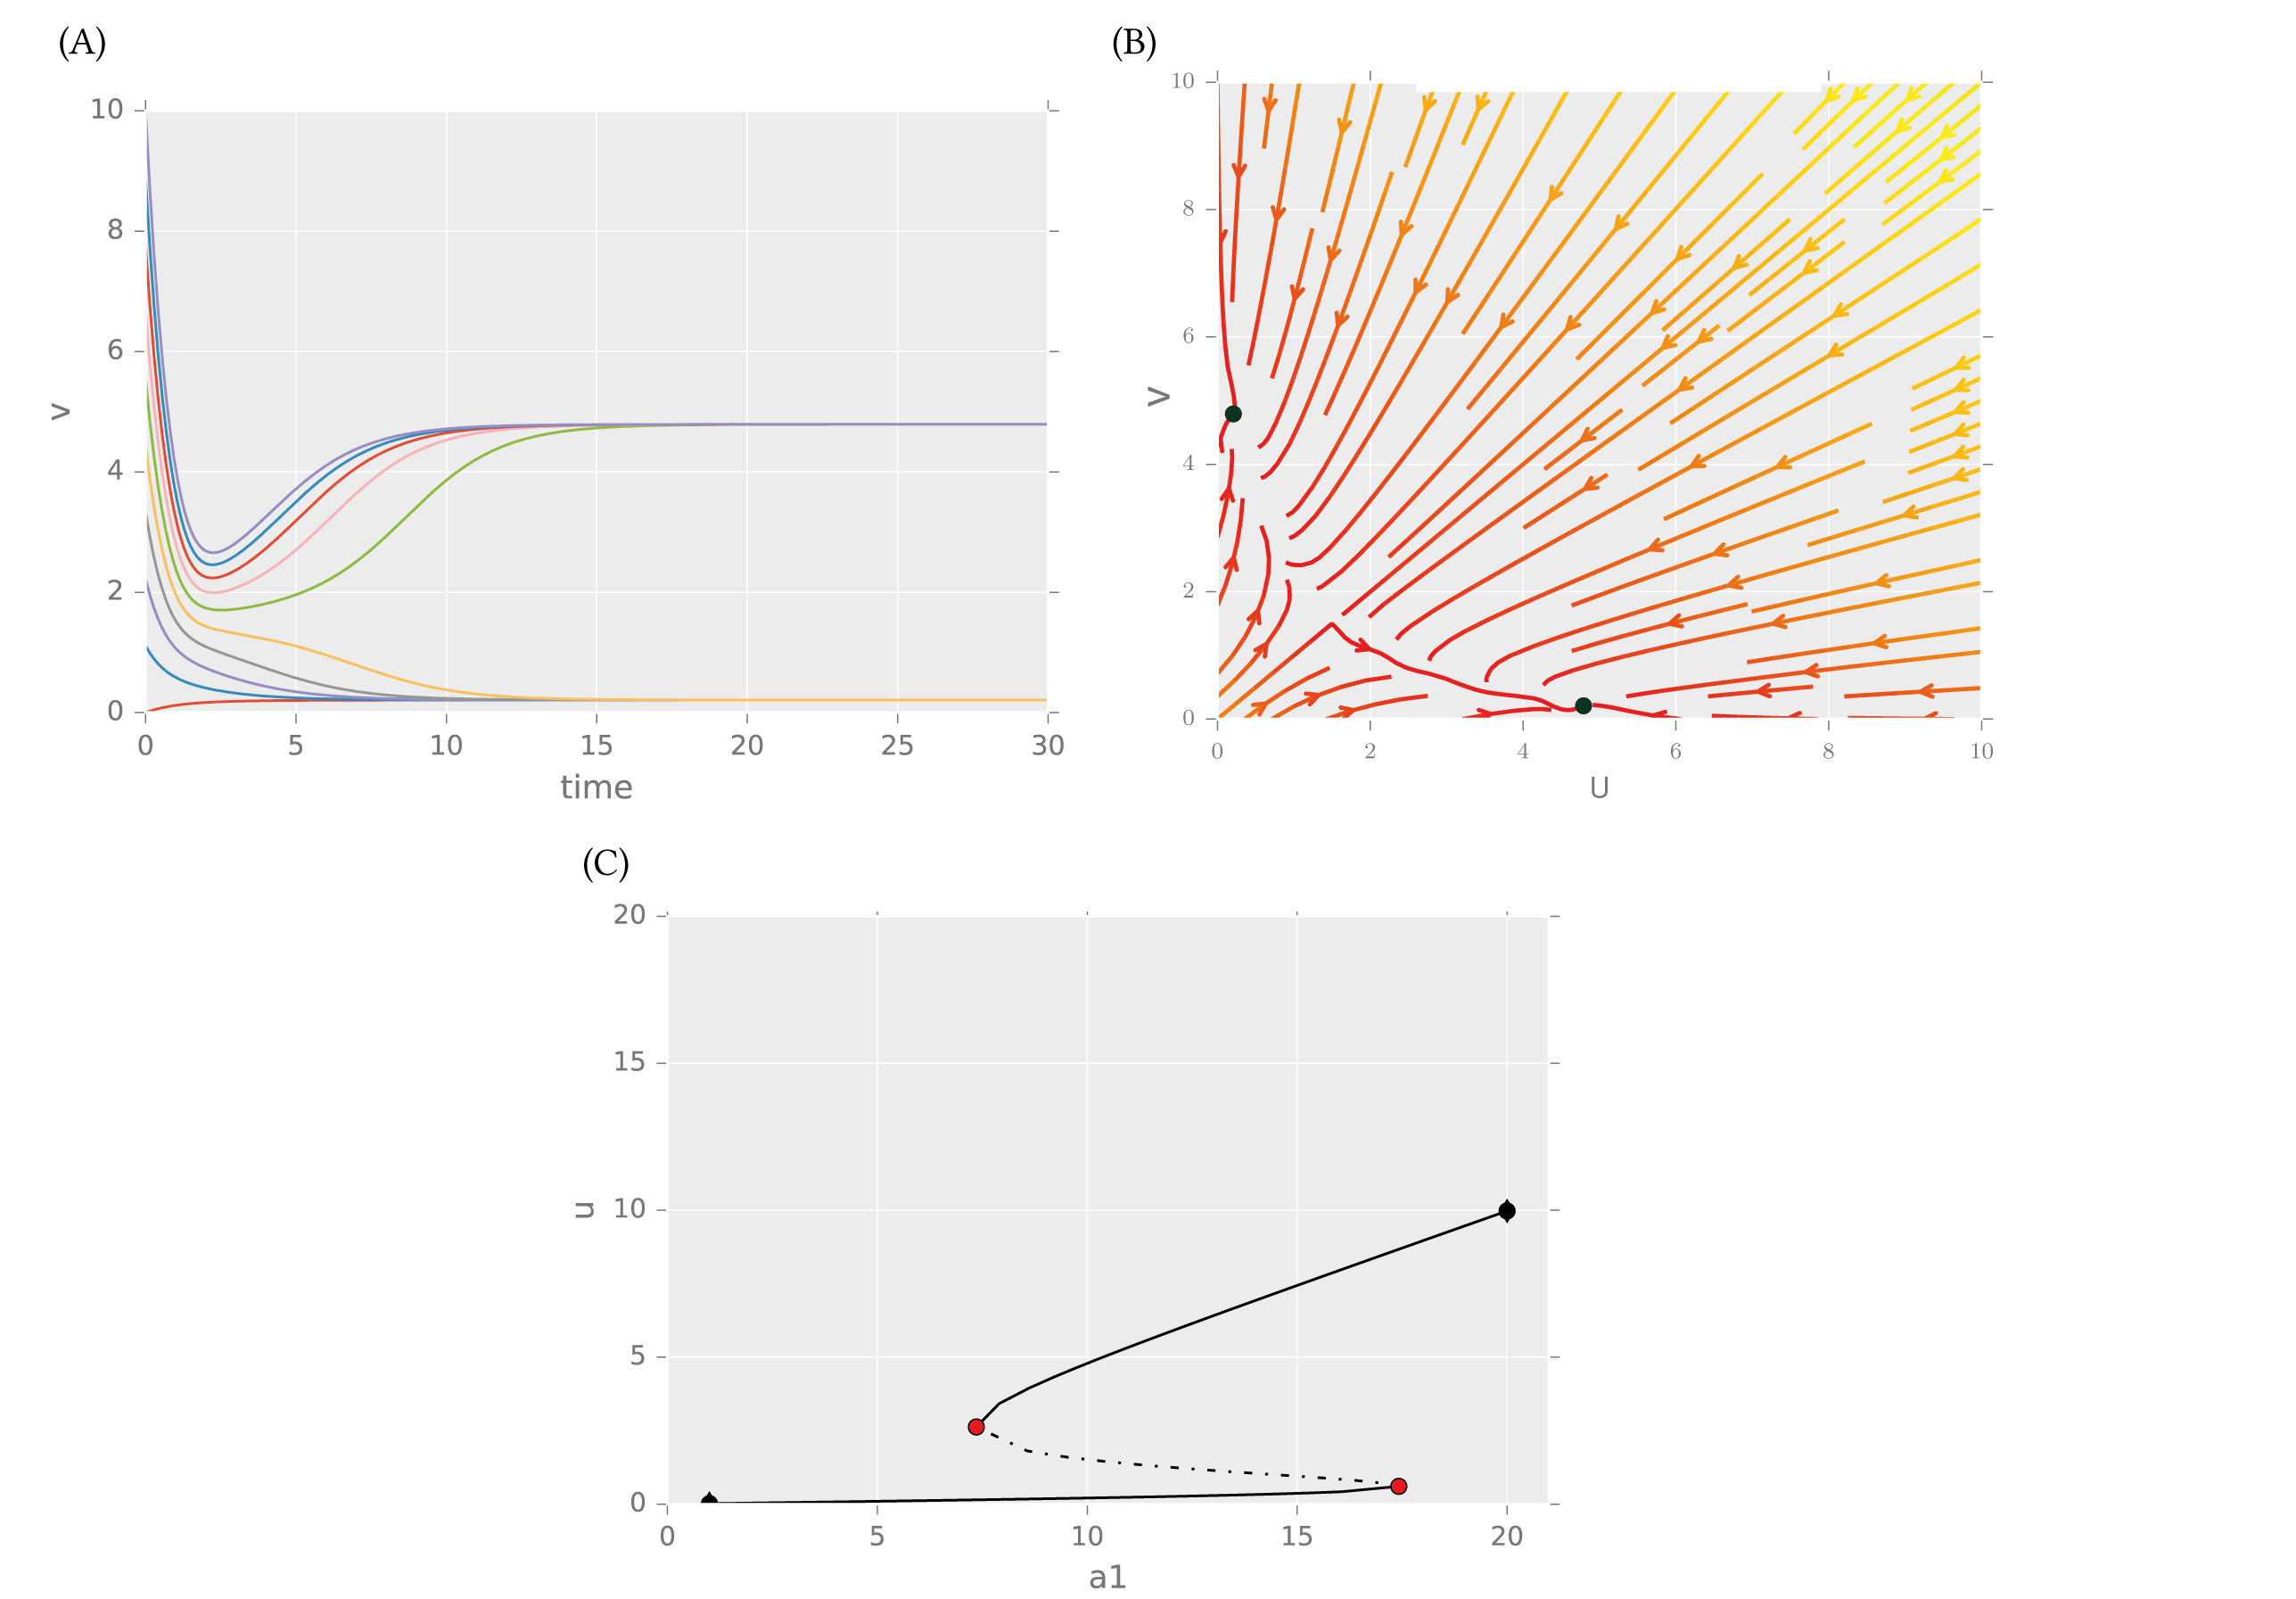
\includegraphics[scale=0.7]{../../chapters/chapterABCSysBio/images/Gard_CS.png}
\caption[LoF caption]{\label{fig:Gard_CS}: The \textcite{Gardner:2000vha} toggle switch is capable of bistable behaviour given $a_1$ and $a_2$ = 10, and β, γ = 2. (A) The timecourse of the simulated model using multiple initial conditions. (B) The vector plot of the Gardner switch shows there are two stable steady states and one unstable steady state. (C) A bifurcation diagram shows that the system is bistable when 5 \ge{} $a_1$ \le{} 31.}
\end{center}
\end{figure*}
\clearpage


\section{Toggle switch parameter scan}
\label{sec:paramscan}
%This bit is from SF chapter as well
In order to study the switch system in a more realistic way, I developed an extension to the ~\textcite{Gardner:2000vha} switch. This new set of switches does not use the \acrfull{qssa} that is often used in modelling the toggle switch. Using mass action, this changes the two-equation system used in Equations~\ref{eq:gards} into a system of 18 equations. The equations describing the system are shown below and illustrated in Figure~\ref{fig:Gard_MA}. The system consists of two genes, gA and gB. The products of the genes homodimerise and mutually repress eachother. There are also two inducers in the system, S and R. S removes AA from the system by binding to the homodimer and thus removes the repression on gene B, and R removes BB from the system by binding to it. A symmetric model, where the parameters for equivalent reactions were set to be the same, was used for simplicity.

\begin{figure*}[tbp]
	\begin{center}
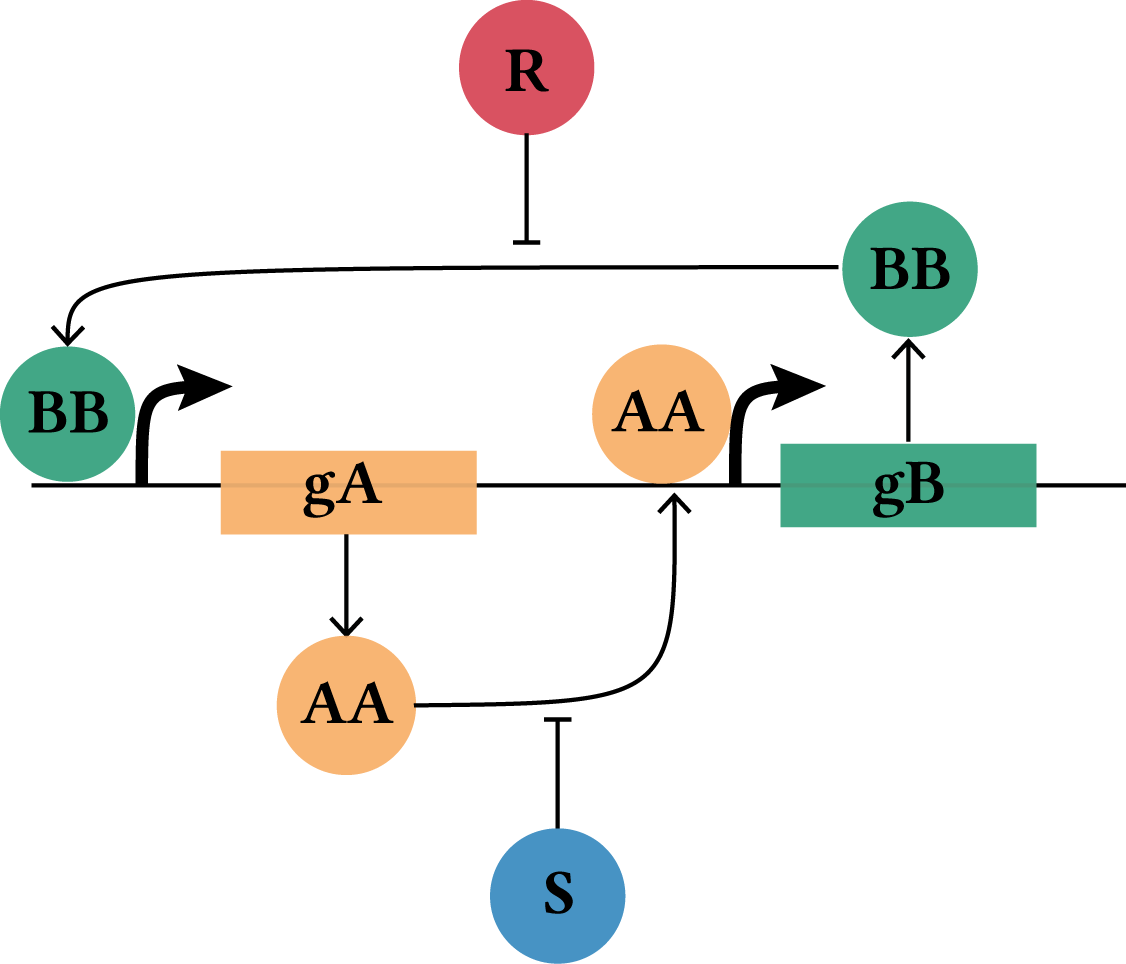
\includegraphics[scale=0.7]{../../chapters/chapterABCSysBio/images/ma-switch-diagram.png}
\caption[LoF caption]{\label{fig:Gard_MA}:An illustration of the model used in the parameter scan. }
\end{center}
\end{figure*}



$$
\begin{array}{cccc}
      \textrm{gA}\stackrel{\textrm{ge}}{\longrightarrow}\textrm{gA} + \textrm{A} \\
      \textrm{gB}\stackrel{\textrm{ge}}{\longrightarrow}\textrm{gB} + \textrm{B} \\
      \textrm{A} + \textrm{A} \stackrel{\textrm{dim}}{\longrightarrow}\textrm{A2} \\
      \textrm{A2} \stackrel{\textrm{dim\_r}}{\longrightarrow}\textrm{A} + \textrm{A} \\
      \textrm{B} + \textrm{B} \stackrel{\textrm{dim}}{\longrightarrow} \textrm{B2} \\
      \textrm{B2} \stackrel{\textrm{dim\_r}}{\longrightarrow}\textrm{B} + \textrm{B} \\
      \textrm{gA} + \textrm{B2} \stackrel{\textrm{rep}}{\longrightarrow}\textrm{B2gA} \\
      \textrm{B2gA} \stackrel{\textrm{rep\_r}}{\longrightarrow}\textrm{B} + \textrm{gA} \\
      \textrm{gB} + \textrm{A2} \stackrel{\textrm{rep}}{\longrightarrow}\textrm{A2gB} \\
      \textrm{A2gB} \stackrel{\textrm{rep\_r}}{\longrightarrow}\textrm{A2} + \textrm{gB} \\
      \textrm{A} \stackrel{\textrm{deg}}{\longrightarrow}\textrm{\O}\\
      \textrm{B} \stackrel{\textrm{deg}}{\longrightarrow}\textrm{\O}\\
      \textrm{S} + \textrm{A2} \stackrel{\textrm{rep\_dim}}{\longrightarrow}\textrm{SA2}\\
      \textrm{SA2} \stackrel{\textrm{rep\_dim\_r}}{\longrightarrow}\textrm{S} + \textrm{A2}\\
      \textrm{R} + \textrm{B2} \stackrel{\textrm{rep\_dim}}{\longrightarrow}\textrm{RB2}\\
      \textrm{RB2} \stackrel{\textrm{rep\_dim\_r}}{\longrightarrow}\textrm{R} + \textrm{B2}\\
      \textrm{R} \stackrel{\textrm{deg}}{\longrightarrow} \textrm{\O}\\
      \textrm{S} \stackrel{\textrm{deg}}{\longrightarrow}\textrm{\O}\\
\end{array}
$$
%This bit is in SF chapter also:
This model is too complex to solve analytically. In order to determine whether it is capable of bistable behaviour, a numerical solution must be deployed. In order to do that I used a parameter scanning algorithm outlined in Algorithm~\ref{alg:param_scan} below. This method involves the scan of parameter values as well as initial conditions for AA and BB. Parameter values are sampled randomly from a uniform distribution. Then for each sample of values, latin hypercube sampling is used to sample initial conditions~\autocite{MCKAY:2000vt}. This is used to ensure that the whole space is sampled uniformly. Latin hypercube sampling is done in two dimensions, in order to sample initial conditions for the two dimers, AA and BB. The uniform priors of the two species in consideration represent a rectangle space, which is subdivided into equal parts. Then a random sample is drawn from each sub-part. This ensures the whole space is evenly sampled. 
\clearpage
\begin{figure*}[tbp]
\begin{center}
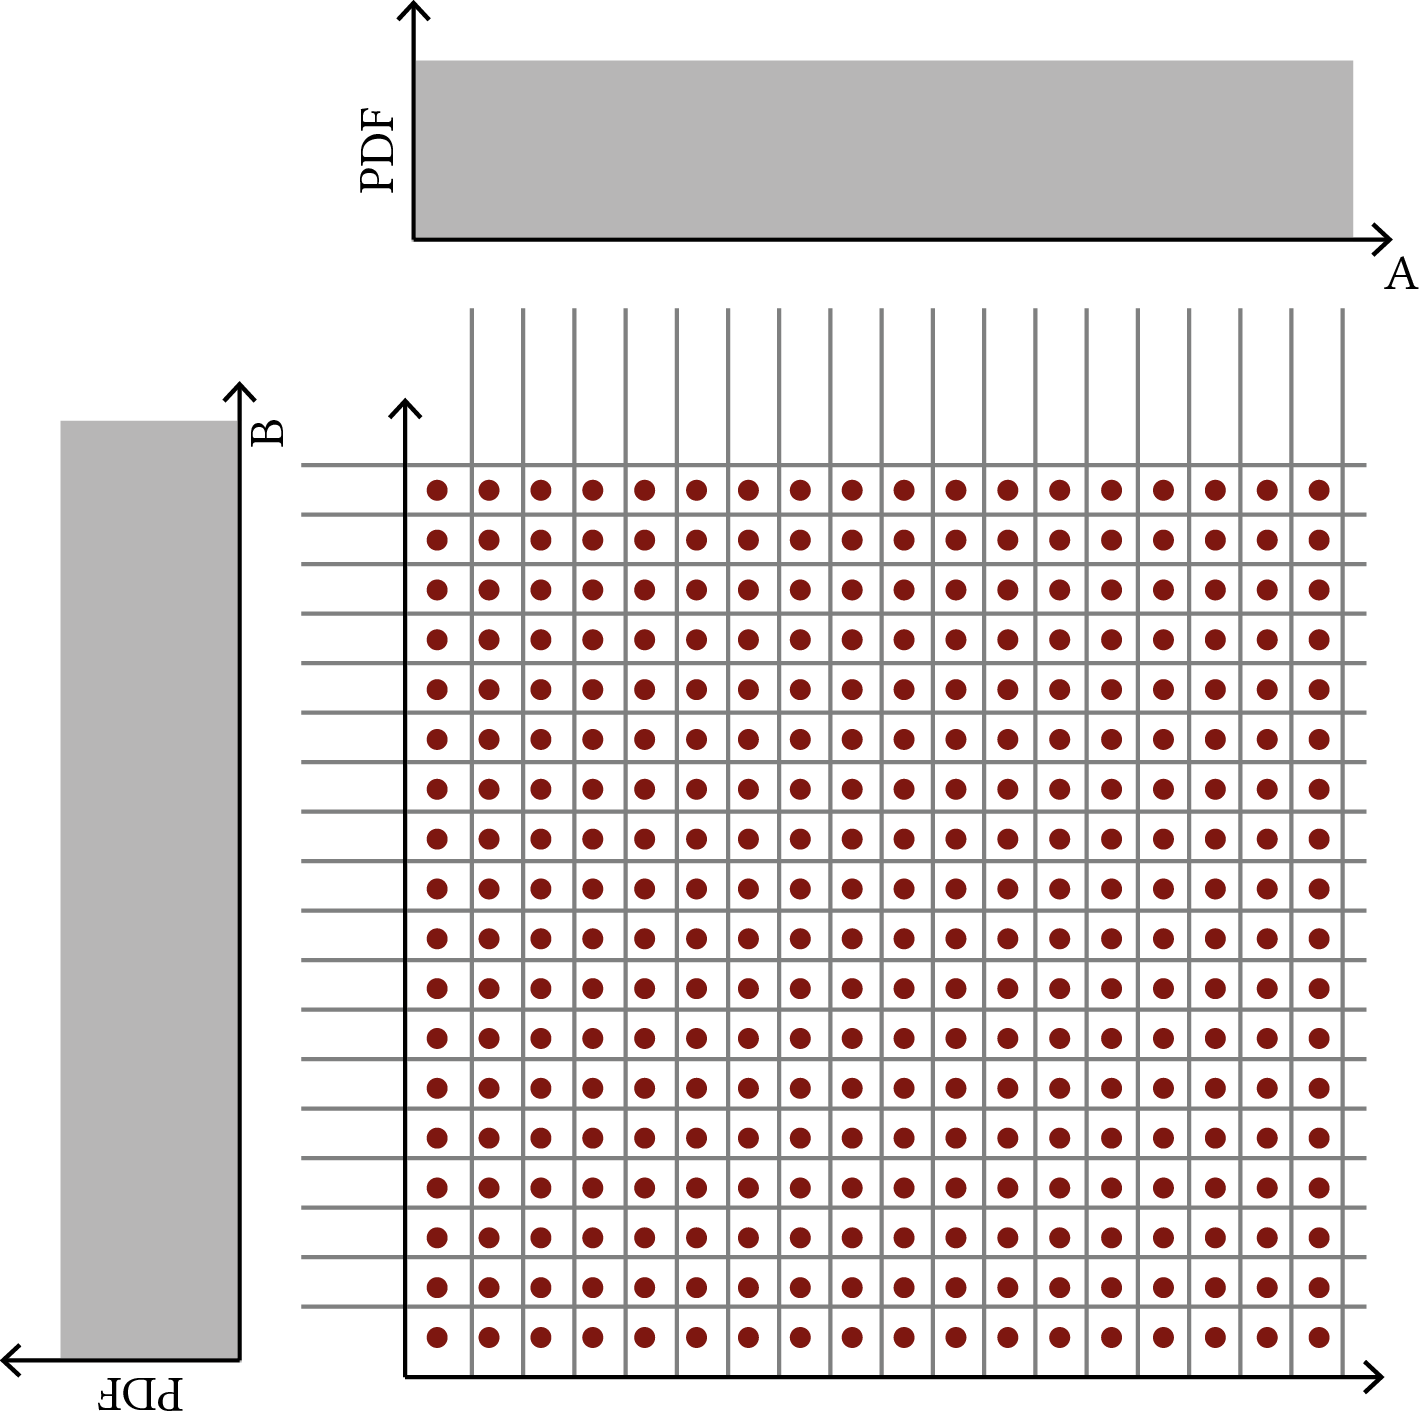
\includegraphics[scale=0.5]{../../chapters/chapterABCSysBio/images/LHS.png}
\caption[LoF caption]{\label{fig:lhs}Latin hypercube sampling ensures that the whole space is sampled evenly. For the two species concerned, A and B, we assume uniform distributions, shown in grey. The joint space of the two distributions is divided into smaller equal parts and a random sample is drawn from within each subspace.  }
\end{center}
\end{figure*}


The parameter scan uncovered the presence of tristable, bistable and monostable systems given a different set of parameter values. The Algorithm of the parameter scans is outlined below:
%A deterministic and a stochastic scan were carried out. 


\begin{algorithm}[htbp]
\caption{Parameter scan algorithm}
\label{alg:param_scan}
 \begin{algorithmic}[1]
    \Statex
	\State Select multiple sets of parameter values from a random uniform distribution between 0 and 10.
	\For{each set of parameter values}:
	\State Select multiple sets of initial conditions for the two dimers via latin hypercube sampling
	\For{For each set of initial conditions}
	\State Integrate ODEs of the model
	\State Solve system to steady state
	\EndFor
	\EndFor
  \end{algorithmic} 
\end{algorithm}

One dimer was plotted against the other for all initial conditions of each parameter set. An example for each of the three types of stabilities found during the scan are shown in Figure ~\ref{fig:stab exampl}.

\begin{figure*}[htbp]
\centering
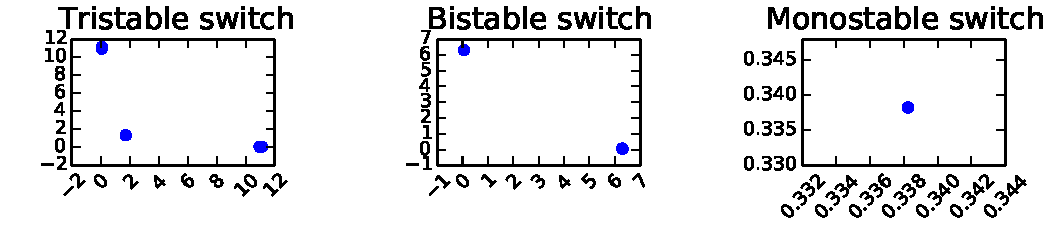
\includegraphics[width=\textwidth]{../../chapters/chapterABCSysBio/images/switch_stbility_examples}
\caption[LoF caption]{\label{fig:stab exampl}: An example for each type of switch found during the parameter scan. Each graph represents the steady state values of one dimer plotted against the other, from one parameter set and 100 initial conditions.}
\end{figure*}



In order to determine which areas in the parameter space give rise to the different kinds of stability, a histogram of the frequency of each parameter value found in monostable, bistable and tristable systems was plotted and shown in Figure~\ref{fig:scan ode param hist}. There were a total of 217 monostable, 16 bistable and 6 tristable switches out of 400 sampled parameter sets. The remaining samples did not reach steady state. This shows that different parameter values have a great effect on the stability profile of the switch.
 
\begin{figure}
\centering
\begin{minipage}[c]{1\textwidth}
\centering
    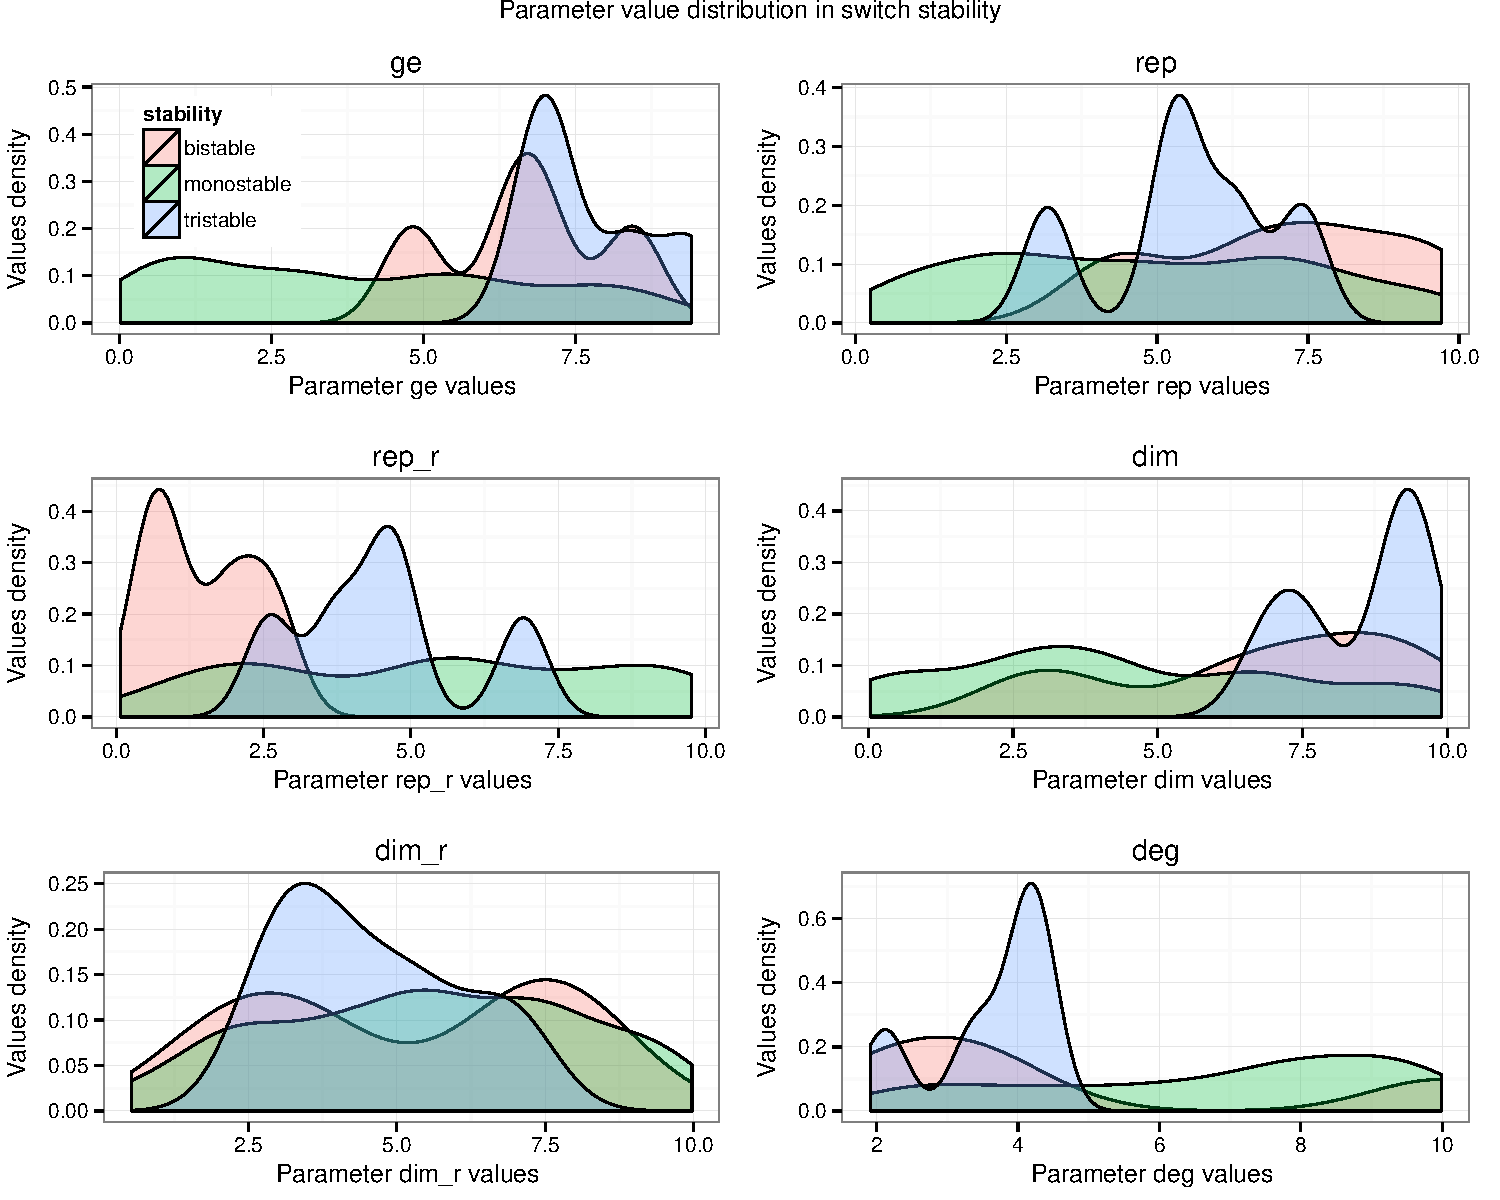
\includegraphics[width=1.05\textwidth]{../../chapters/chapterABCSysBio/images/param_stability_hist}
    \caption{The distribution of parameter values that resulted in monostable, bistable and tristable switches in the parameter scan. Each graph represents the distribution of the values of one parameter. }
    \label{fig:scan ode param hist}
\end{minipage}
\end{figure}


From the histograms in Figure ~\ref{fig:scan ode param hist} it can be seen that the parameter for gene expression (ge) tends to be relatively high when bistability arises whereas the parameter for the reverse reaction of repression (rep\_r) tends to be low. Degradation (deg) also tends to be low. It must also be noted that the parameter values that give rise to monostable systems are generally evenly distributed for all parameters, suggesting that monostable systems arise from the whole range of values sampled. This can further indicate that the right combination of more than one parameter values is necessary for bistability. 



\section{Toggle switch parameter inference}


In this section I study the problem of how to rationally design a synthetic biological system to perform a behaviour of choice.  In order to address this question I use a Bayesian approach, known as \acrlong{abc} and described in Section(XXX). This approach is capable of approximating the posterior distribution that gives rise to the behaviour of choice~\autocite{Toni:2009tr}. By simulating the model in question, this approach can identify an approximate posterior distribution via a series of intermediate distributions. Here I use an implementation of the above approach, the software package ABC-SysBio~\textcite{Liepe:2010eg}. This method can be used for the rational design of synthetic biological systems by defining some design objectives to which the model is fitted to~\textcite{Barnes:2011hh}. By specifying the inputs to the system and the outputs required, the posterior of the model that can produce this behaviour can be identified. 

This method is used here to fit the model used in Section~\ref{sec:paramscan} to a switch-like behaviour. The design specifications are shown in Figure~\ref{fig:abc_behav}. The two inducers, S and R, as used as inputs to flip the switch ON and OFF respectively. The required output is the switch flipping from the OFF state to the ON state and then to the OFF state again. As priors to the parameter inference I used the parameter values shown to produce a bistable switch in Section~\ref{sec:paramscan}. The priors used are shown in Table~\ref{tab:param_inf_params}.

\begin{table}[htbp]
\centering
\caption{The parameter priors used for the standard toggle switch parameter inference. The priors consist of the lower and upper limit of a uniform distribution}
\label{tab:param_inf_params}
\begin{tabular}{ccccccccc}
\toprule
 \textbf{ge}     & \textbf{rep}     & \textbf{rep r}     & \textbf{dim}    & \textbf{dim r}     & \textbf{deg}  & \textbf{rep dim}    & \textbf{rep dim r} & \textbf{deg sr}    \\
6 9     & 4 10    & 1 4       & 4 10   & 2 7       & 2 5  & 0.05 0.1   & 0.01 0.05     & 0.01 0.05         \\ \bottomrule
\end{tabular}
\end{table}


\begin{figure*}[htbp]
	\begin{center}
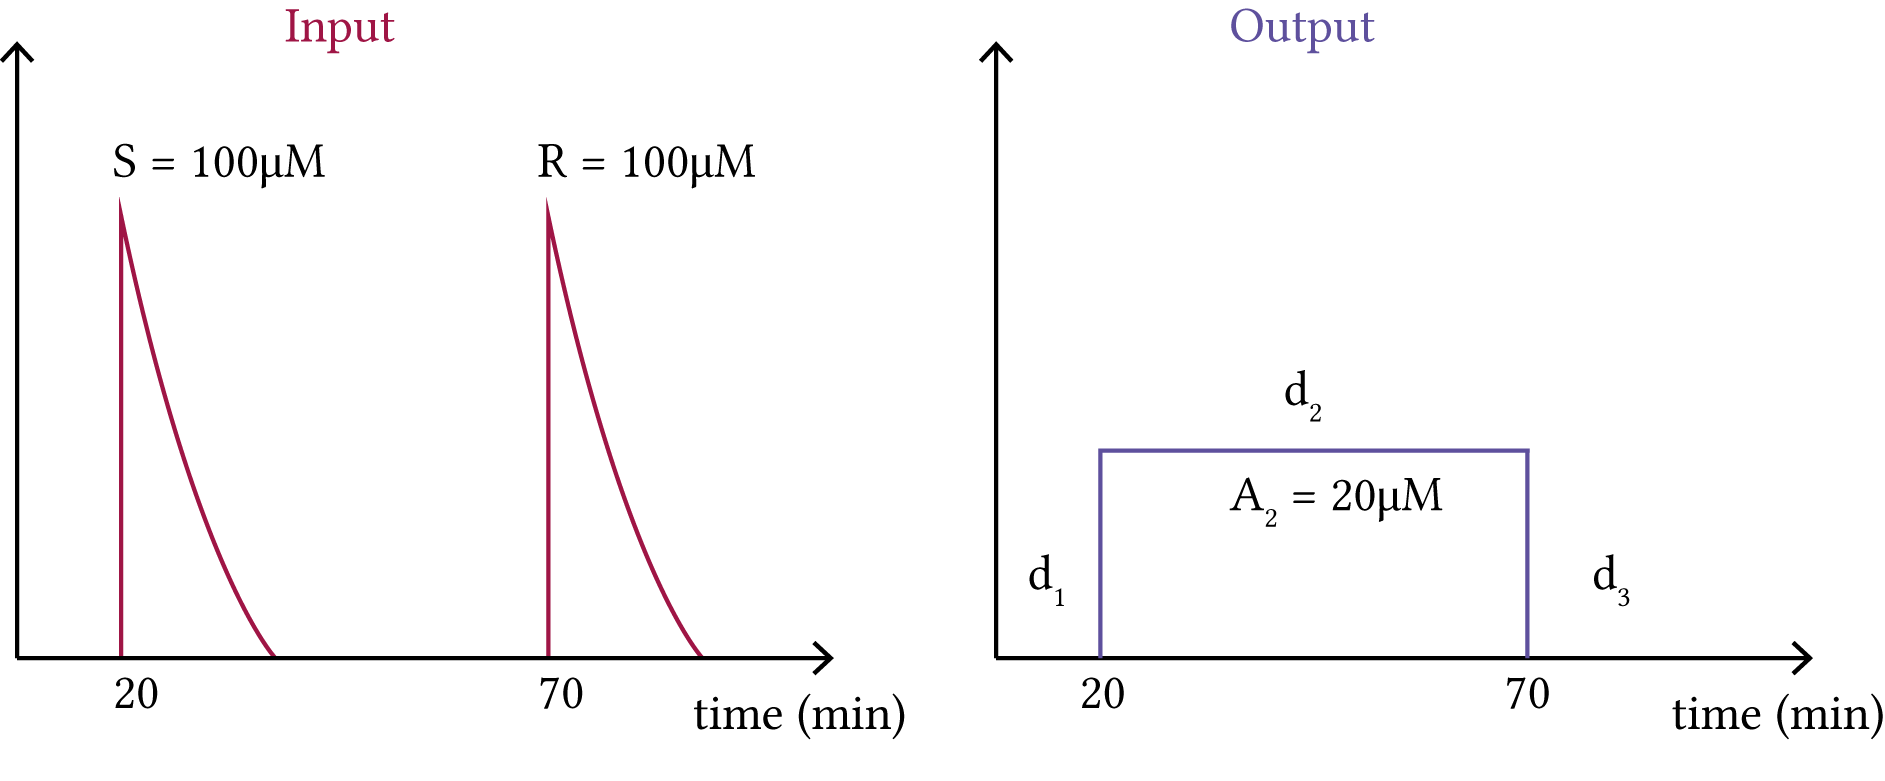
\includegraphics[scale=0.7]{../../chapters/chapterABCSysBio/images/behaviour.png}
\caption[LoF caption]{\label{fig:abc_behav}: Design specification for ABC parameter inference. The input to the system consists of an event turning on the stimulus (S) at t=20 and another turning on the repressor (R) at t=70. The output specification is the response to the switch to these stimuli.}
\end{center}
\end{figure*}
In order to fit the switch model to the behaviour specified above, a distance function must be defined. The distance function defines the quantity that is minimized at each successive iteration of \acrshort{abc} \acrshort{smc}. The distance function defined here is shown in Equations\ref{eq:dist}. Three distances are measured, one for each state of the switch, OFF-ON-OFF.


\begin{align}\label{eq:dist}
	d_1 &= \sum_{i=0}^{20} (s_i-t_1)^2 \\
	d_2 &= \sum_{i=21}^{70} (s_i-t_2)^2 \\
	d_3 &=  \sum_{i=71}^{100} (s_i-t_3)^2,
\end{align}
where $i$ represents the timepoints, $s_i$ the simulation result at  each timepoint and $t1 = 0$, $t2 = 20$, $t3 = 0$ represent each target behaviour.


The result of the toggle switch parameter inference are shown in Figure~\ref{fig:stand_abc_timeseries}. The results show that the model can indeed behave like a switch within the parameter range given as priors. 

\begin{figure}[htbp]
    \centering
    \hspace*{-1cm}
    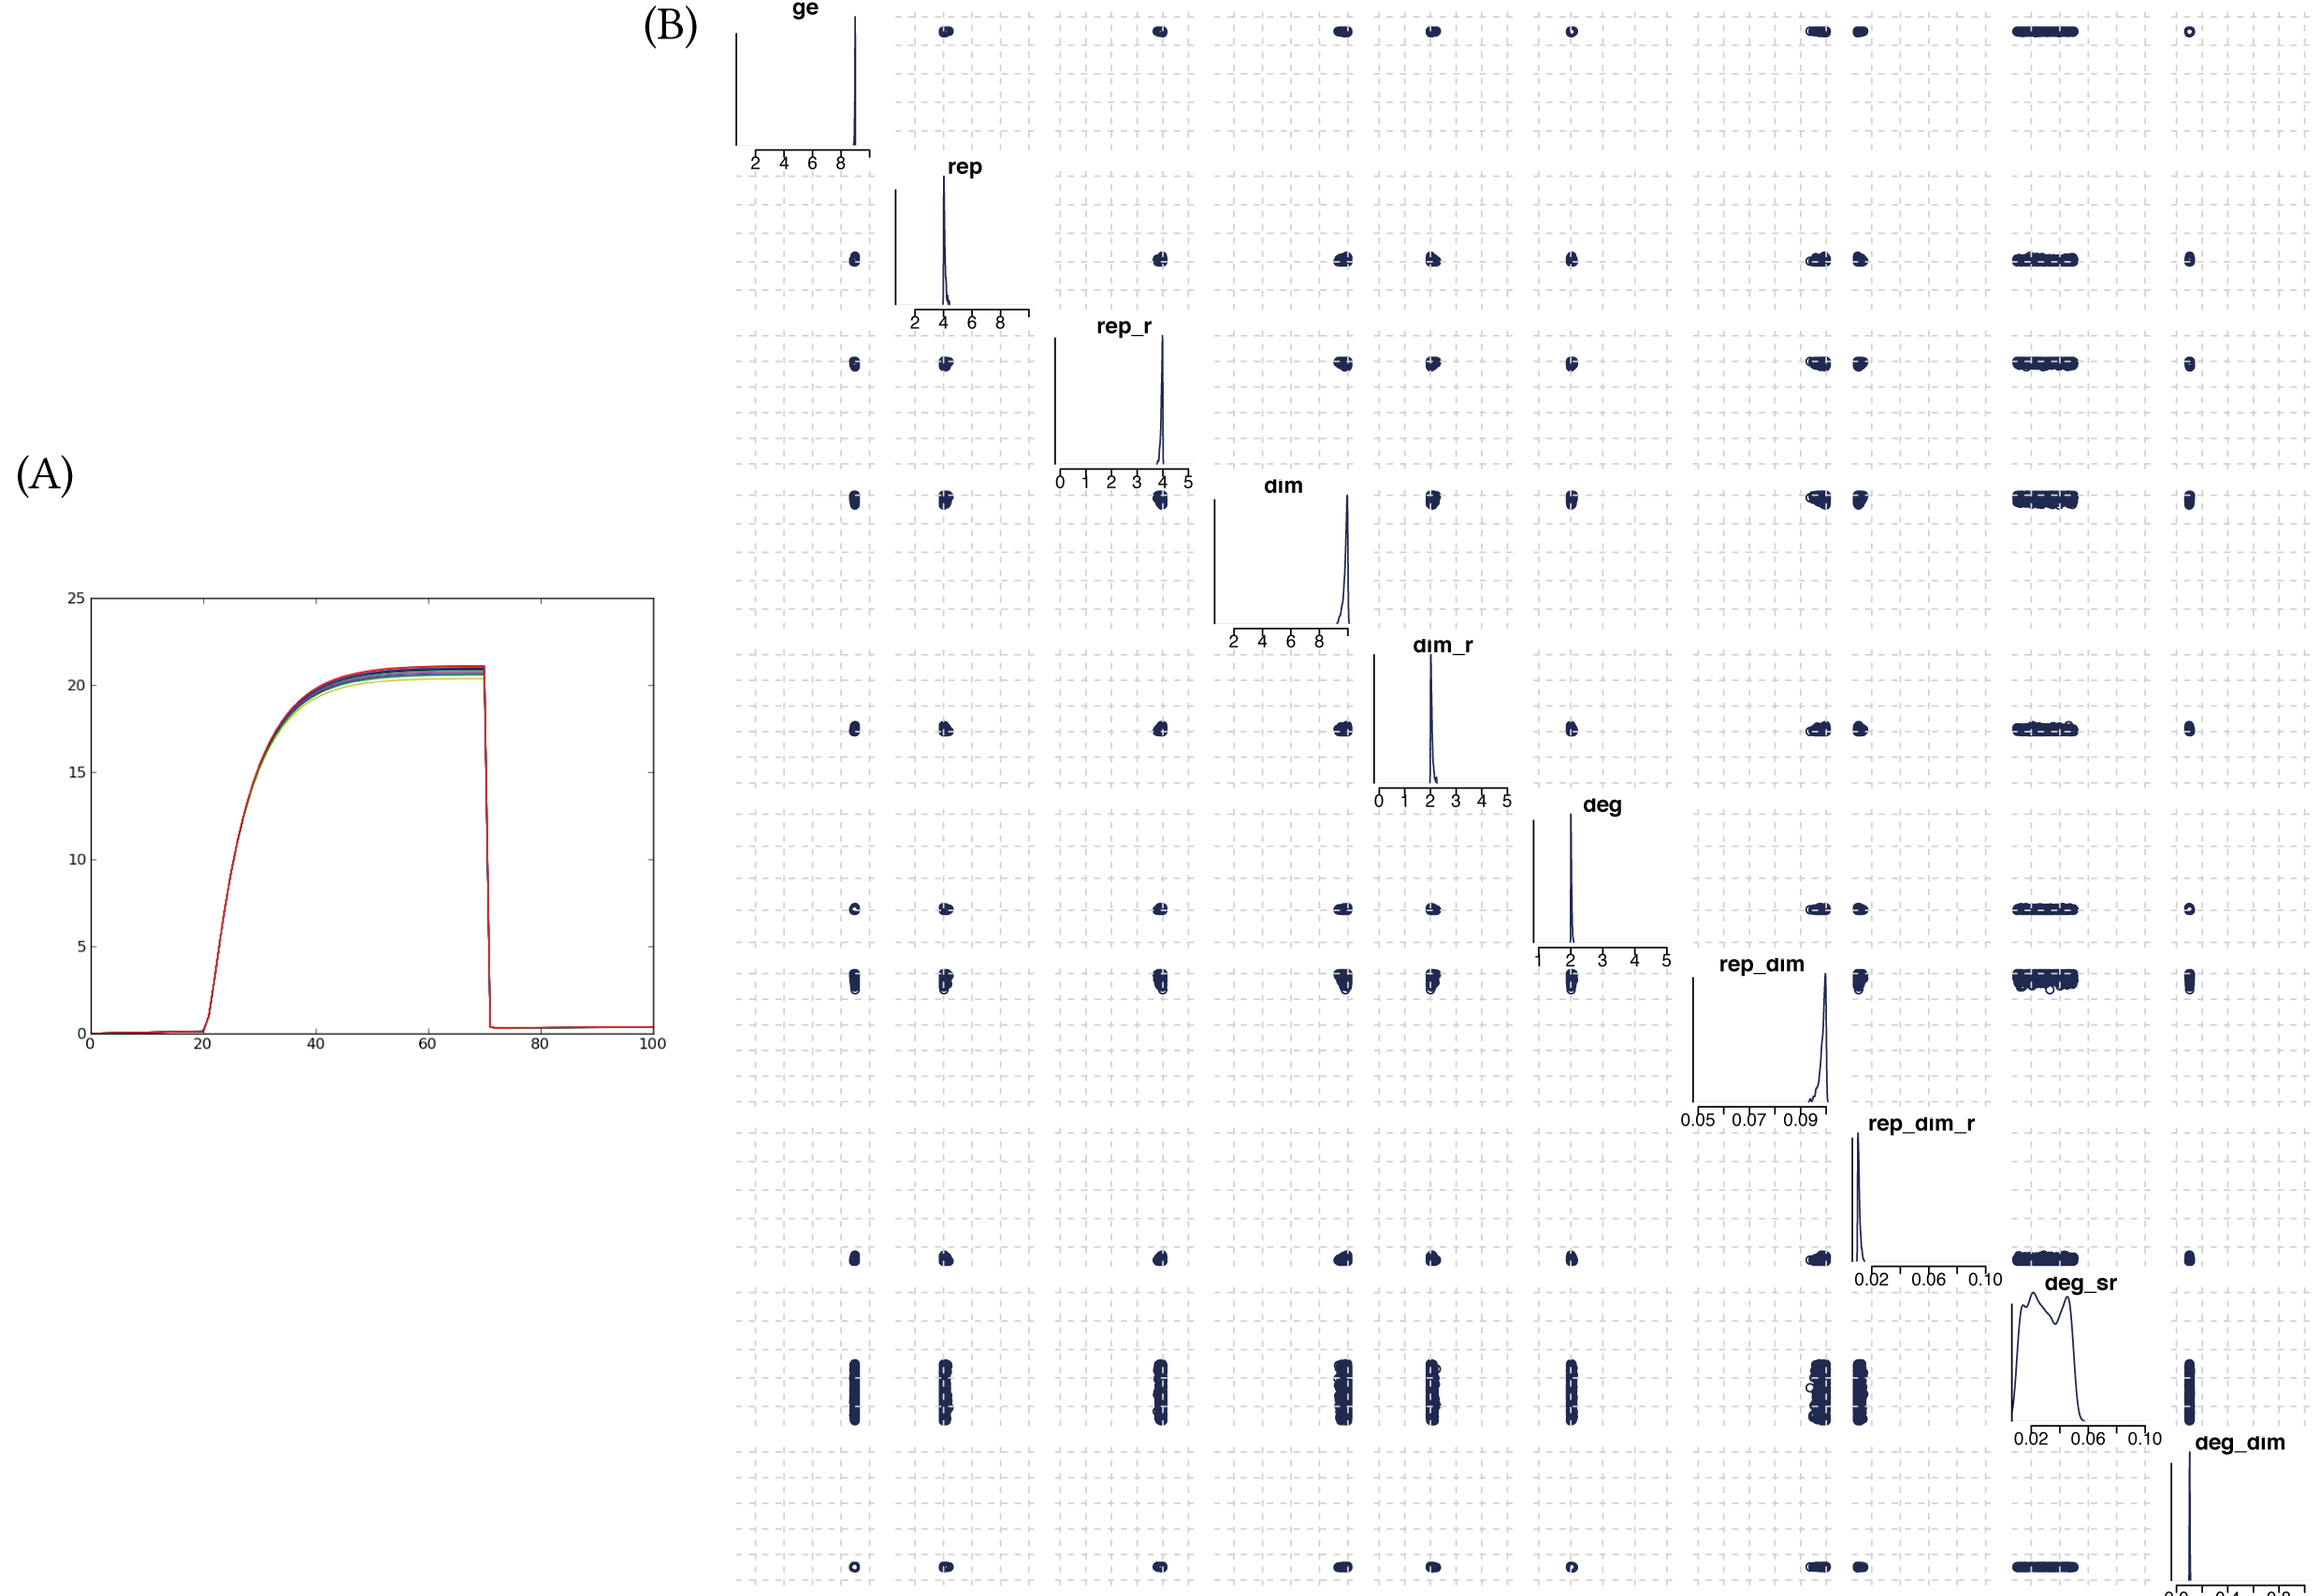
\includegraphics[scale=0.7]{../../chapters/chapterABCSysBio/images/param_inf_res.png}
    \caption{(A) The time series of the final population (for final $\epsilon$ = 2 ) of the standard toggle switch ABC-SMC parameter inference. The stimulus, that represses A2, is added at t=20 and the repressor, that represses B2 is added at t=70. (B) The posterior distribution of the toggle switch.}
    \label{fig:stand_abc_timeseries}
\end{figure}
\clearpage
    

The standard toggle switch model was shown to successfully behave like a switch within the parameter range used here.  By examining Figure~\ref{fig:stand_abc_timeseries}B, I conclude that for this model to behave like the design principles defined, gene expression (ge) must be high relative to the prior. Repression (rep) and degradation must both be low and the rate of dimerisation (dim) must be high relative to the prior. These specifications will be useful when building such a switch in the lab, as the appropriate components must be tweaked. More generally, it can be seen in Figure~\ref{fig:stand_abc_timeseries}B, that the posterior distribution that can produce such a behaviour is narrow, which means there is a small combination of parameter values that can produce this behaviour. In the next section I will examine wether the addition of feedback loops can increase the volume of the posterior that produces the required behaviour.


\section{Genetic toggle switch model selection}

In this section I examine wether the addition of feedback loops to the toggle switch can increase its robustness to parameter fluctuations. It is well known that additional feedback interactions can increase robustness to  noise. 

\subsection{Models of the genetic toggle switch}
\label{sec:models_bist}

I consider 7 models for their capability to behave like a switch. The simple toggle switch, switches with positive autoregulation in either or both nodes and switches with negative autoregulation in either or both nodes. The models considered are illustrated in Figure~\ref{fig:toggle_switch_designs}. 


In order to use these models for model selection, it must first be determined whether they are capable of behaving like a switch. ABC model selection is used to select models that can produce the same behaviour, over a greater range of parameter values. If a model is not capable of producing the desired behaviour for the prior range, then it will not be used for model selection. In order to study each model I built extensions to the ~\autocite{Gardner:2000vha} toggle switch in order to incorporate positive and negative feedback to the system.  The models for the double autoregulation models are shown below. For the single autoregulation models, the unnecessary autoregulation term is set to 0.

Double positive autoregulation: 
\begin{align}\label{eq:gards_neg}
\frac{du}{dt} &= \frac{a_1}{1+v^{\beta} + k_{u}^{\delta_{u}}} - u \\
\frac{dv}{dt} &= \frac{a_2}{1+u^{\gamma }+ k_{v}^{\delta_{v}}} - v,
\end{align}

Double negative autoregulation: 
\begin{align}\label{eq:gards_pos}
\frac{du}{dt} &= \frac{a_1+ k_{u}^{\delta_{u}}}{1+v^{\beta}} - u \\
\frac{dv}{dt} &= \frac{a_2+ k_{v}^{\delta_{v}}}{1+u^{\gamma }} - v,
\end{align}

where $k$ represents the effective binding of the transcription factor to its own promoter and $\gamma$ represents the polymerisation of the bound transcription factor. 


\begin{figure*}[htbp]
	\begin{center}
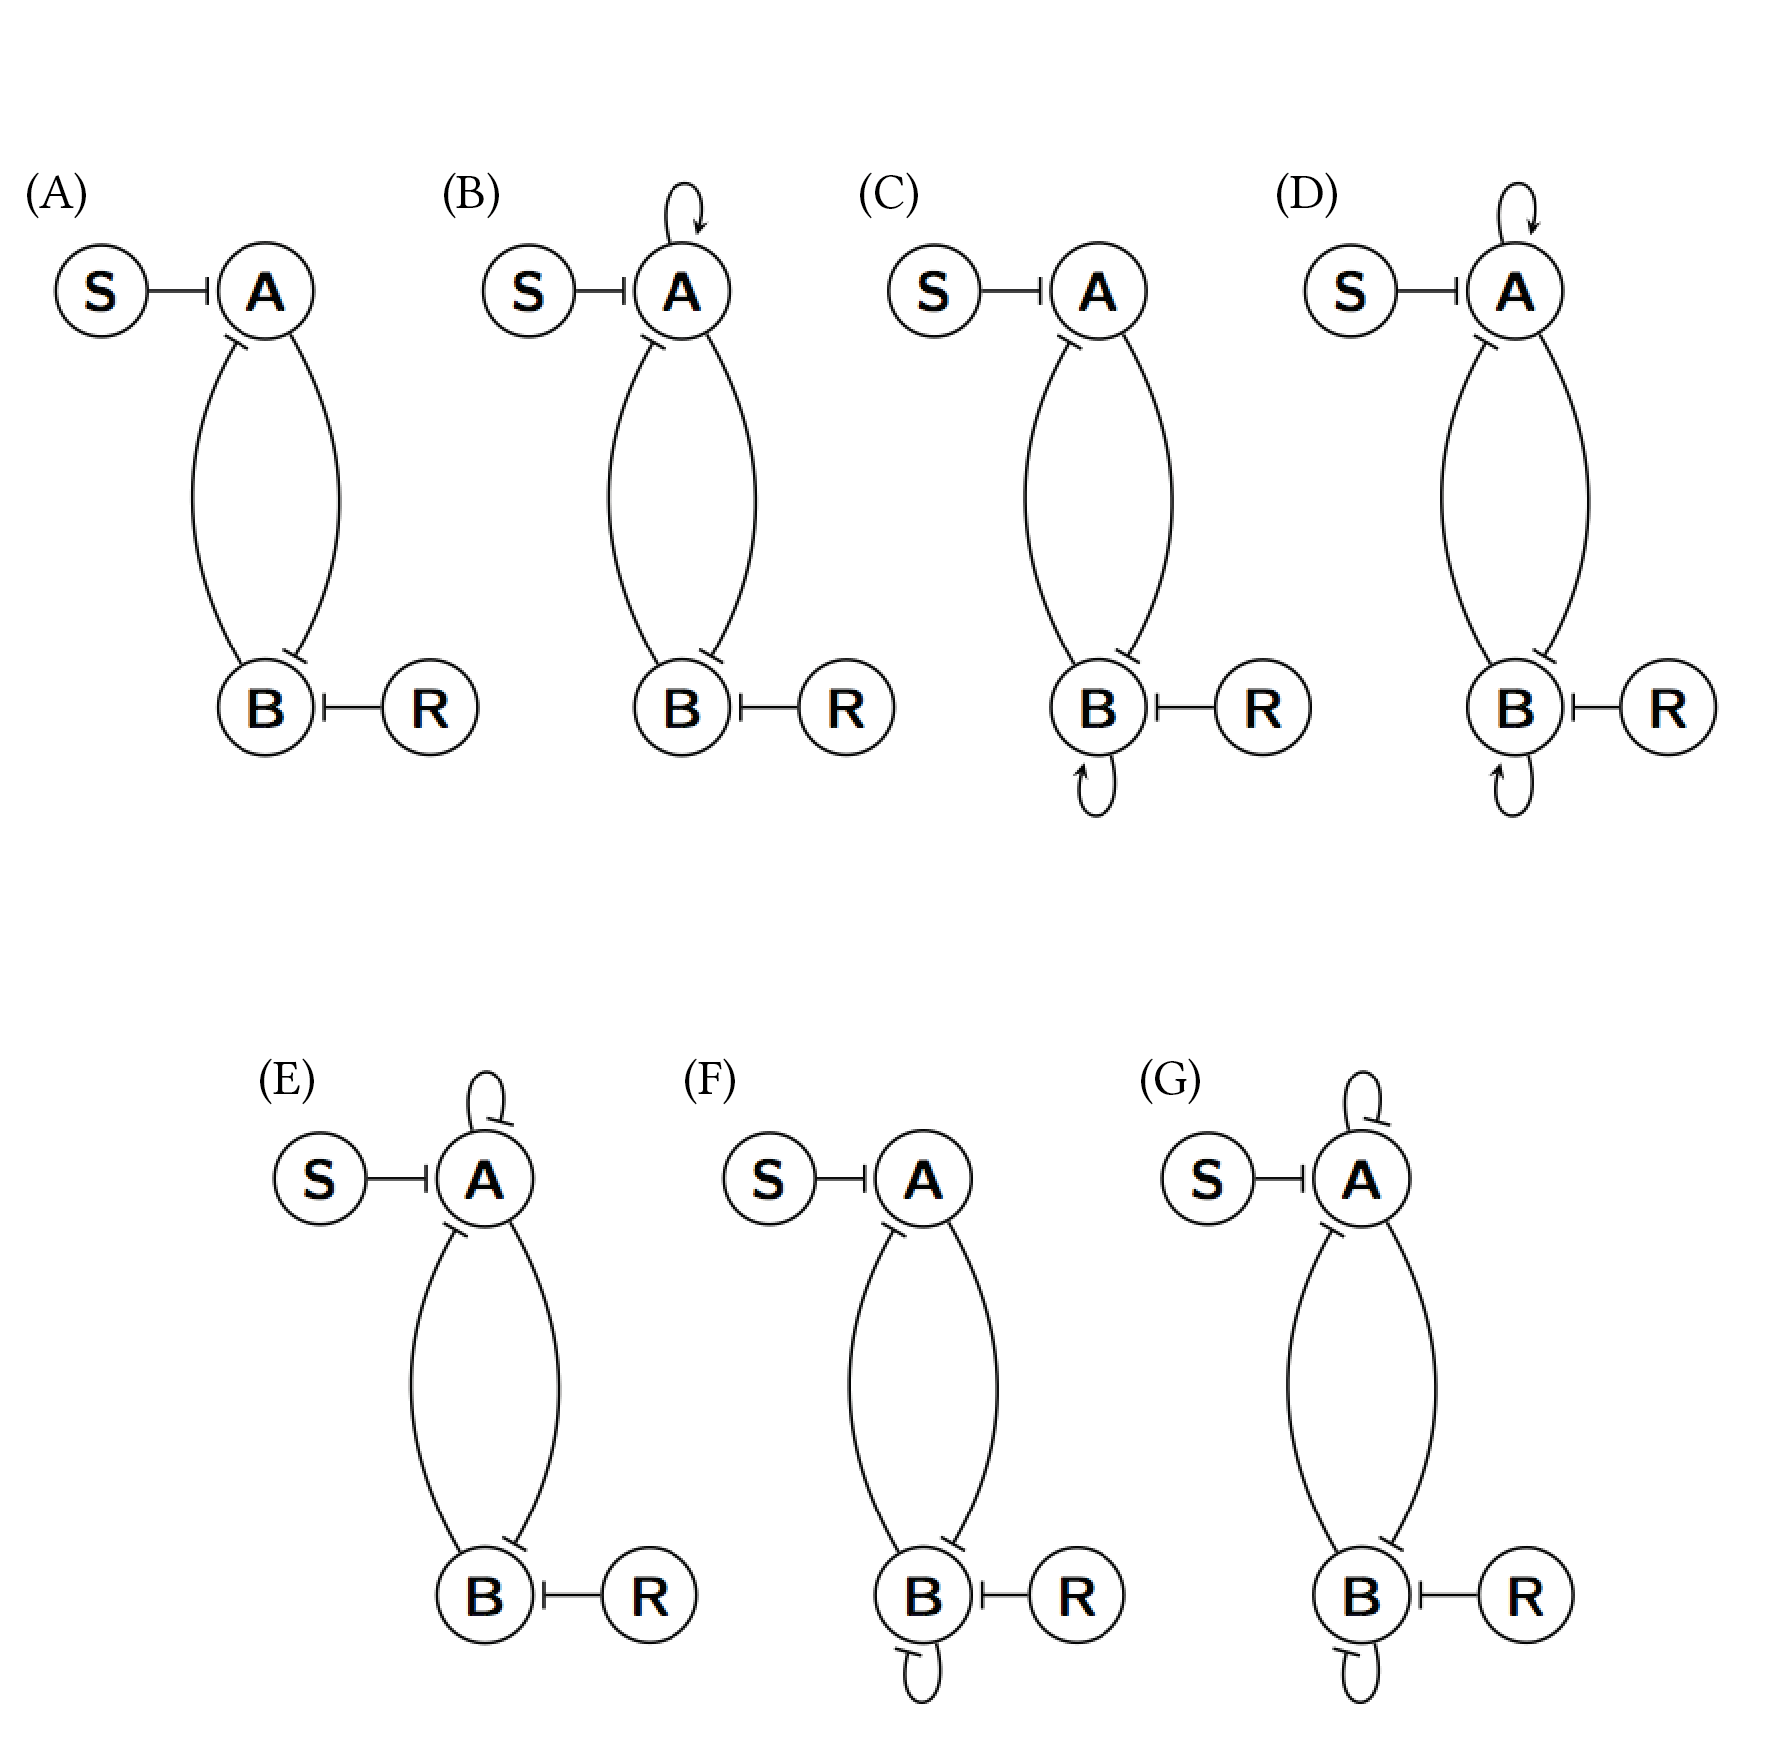
\includegraphics[width=\textwidth]{../../chapters/chapterABCSysBio/images/toggle_switch_designs.png}
\caption[LoF caption]{\label{fig:toggle_switch_designs}: Toggle switch designs considered for model selection}
\end{center}
\end{figure*}
\clearpage


I used the PyDSTool~\autocite{Clewley:2012kj} in order to determine whether each of the 7 switches is capable of bistable behaviour. As shown in Figure~\ref{fig:Gard_pos}, both single and double positive autoregulation is consistent with bistable behaviour. Two stable and one unstable steady state were found for both cases when $k$ = 2 and $\gamma$ = 1. 


\begin{figure*}[htbp]
	\begin{center}
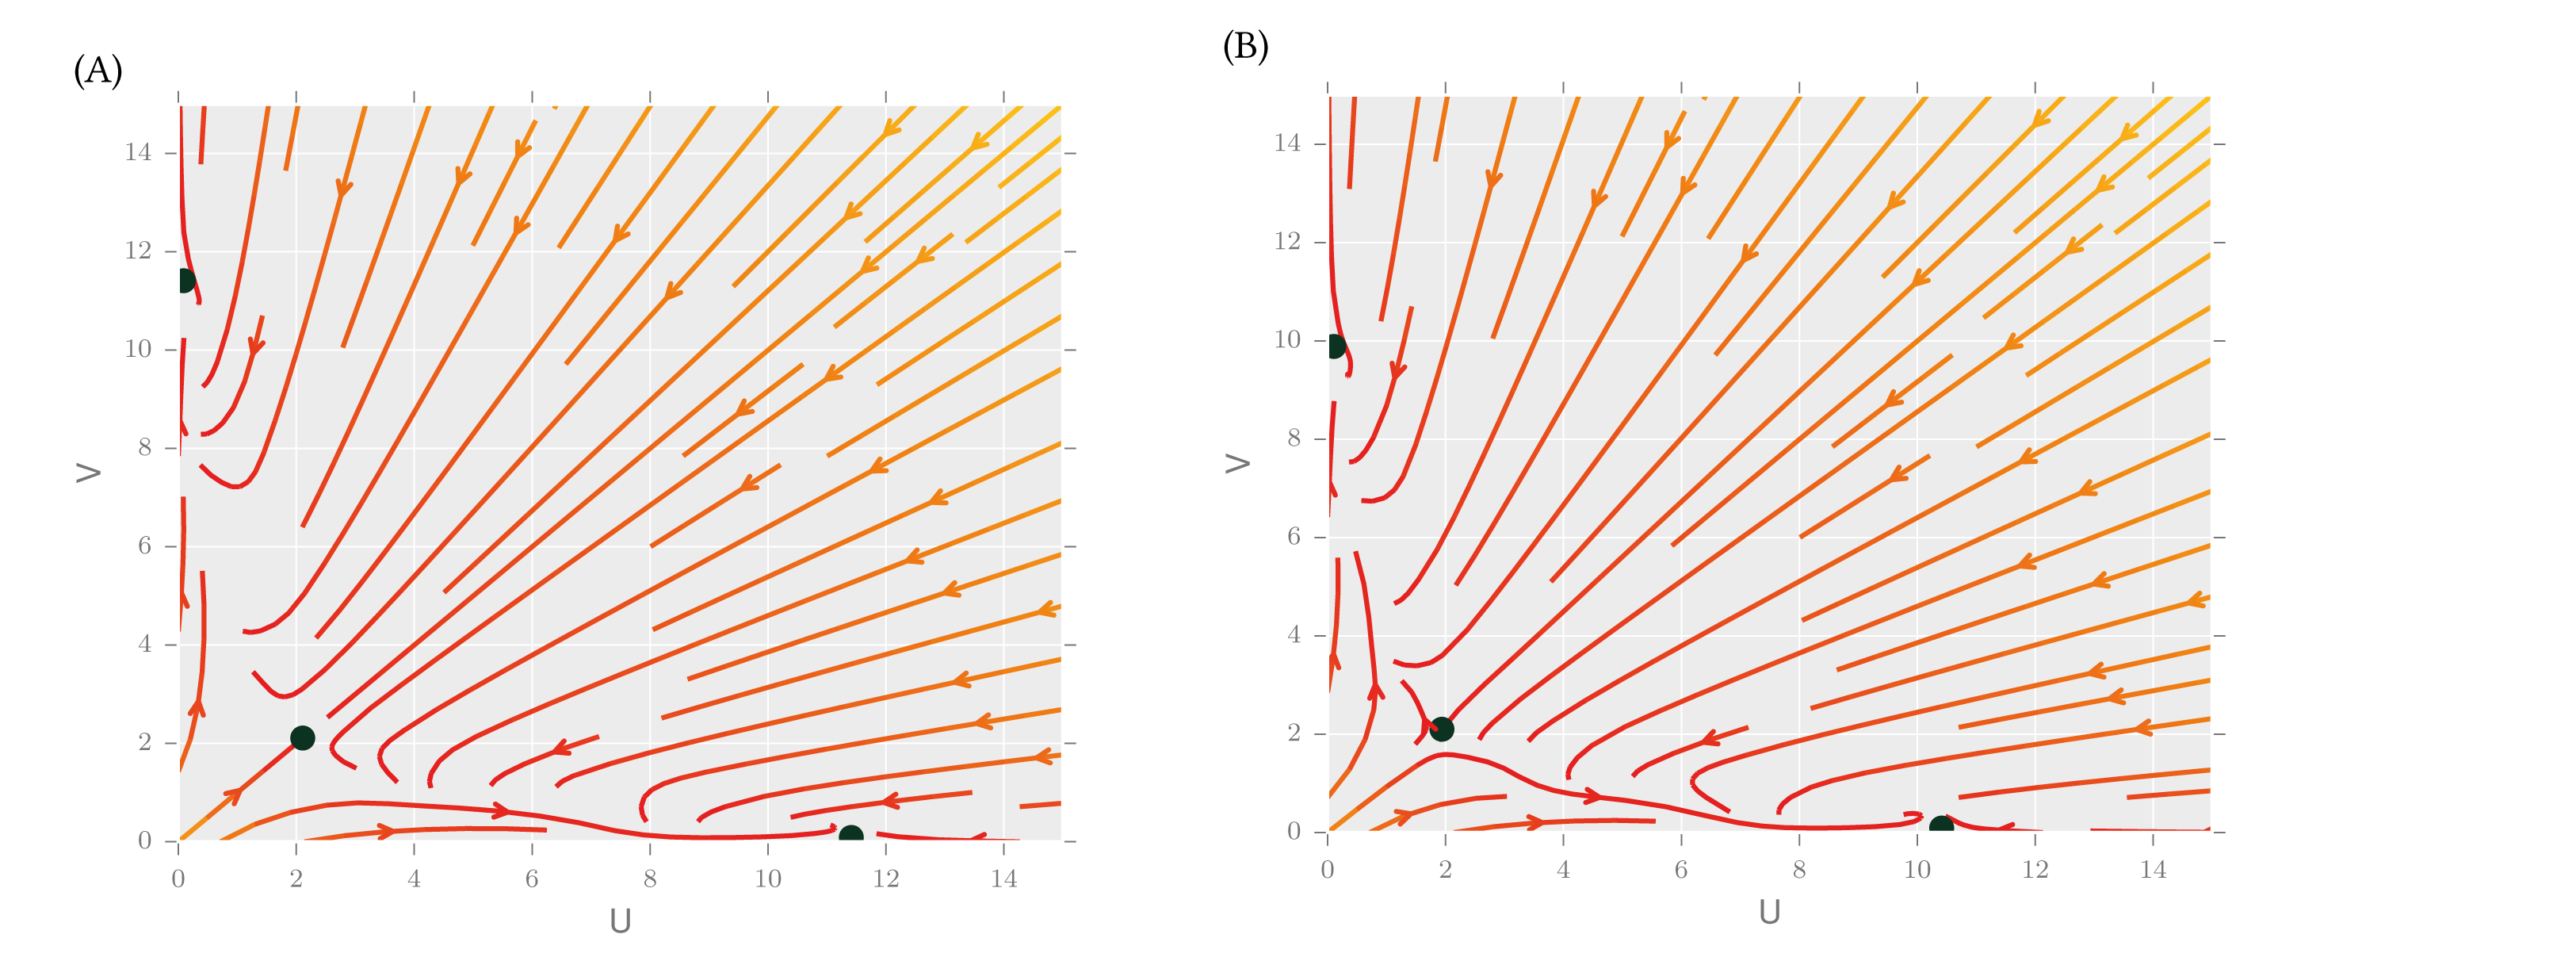
\includegraphics[scale=0.6]{../../chapters/chapterABCSysBio/images/gard_pos.png}
\caption[LoF caption]{\label{fig:Gard_pos}: Both single and positive autoregulation is consistent with bistable behaviour. Two stable and one unstable steady state is found for each model. (A) Single positive autoregulation and (B) double positive autoregulation vector plots.}
\end{center}
\end{figure*}

On the other hand, negative autoregulation was not consistent with bistable behaviour. A bifurcation analysis, when all other parameters are kept constant and only $k$ varied, shows that  even small values of $k$ destroy bistability. This is shown in Figure~\ref{fig:Gard_neg}C. 
\begin{figure*}[htbp]
	\begin{center}
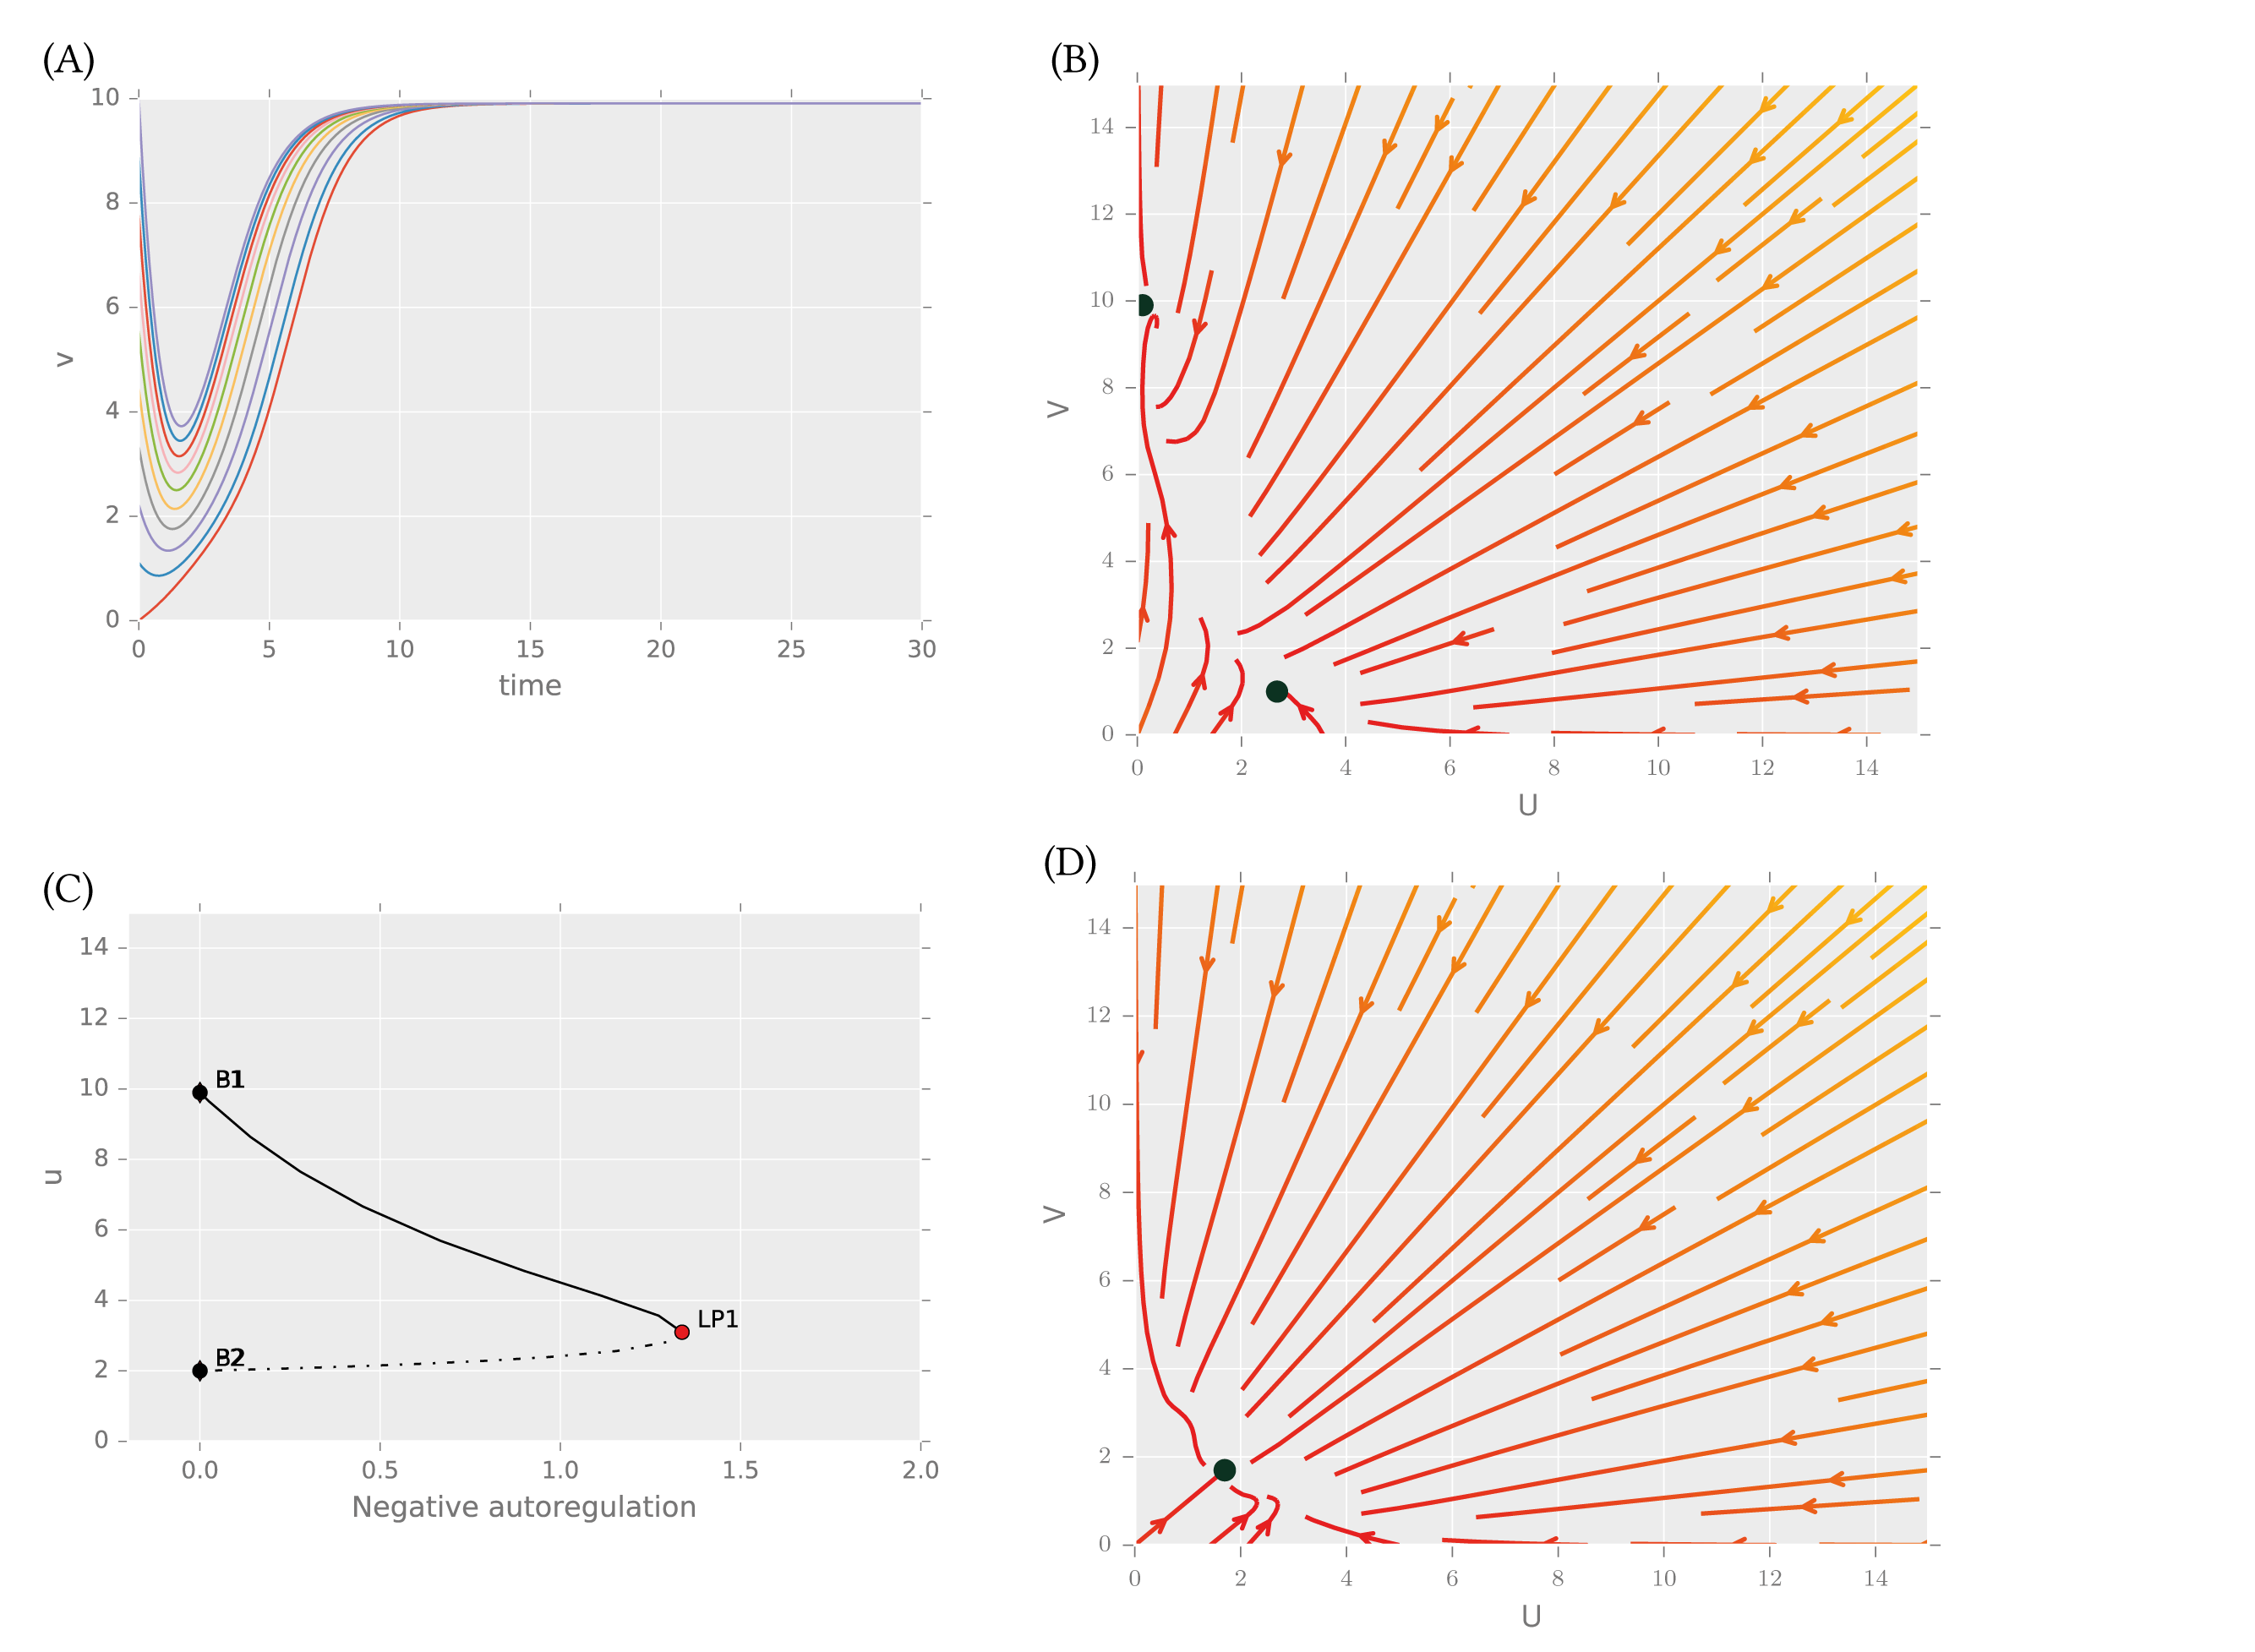
\includegraphics[scale=0.7]{../../chapters/chapterABCSysBio/images/gard_neg.png}
\caption[LoF caption]{\label{fig:Gard_neg}:(A) Timecourse of the single negative autoregulation switch, when $k_u$=2 with varying initial conditions. The system is monostable. (B) One stable and one unstable steady states are found for the single negative autoregulation switch when $k_u$=2 (C) Bifurcation diagram of the single positive autoregulation switch, where all parameters remain constant and only $ku$ varied. (D) The vector plot of the switch with double negative autoregulation. The switch is monostable.}
\end{center}
\end{figure*}




\clearpage




%the rational comparison of models under parameter uncertainty using Bayesian model selection, which automatically accounts for model complexity (number of parameters) and robustness to parameter uncertaint


\subsection{\acrlong{abc} for model selection}

Using the models shown in Section~\ref{sec:models_bist} to exhibit bistability, model selection is carried out. Bayesian model selection is used to directly compare the competing designs using ABC-SysBio~\autocite{Liepe:2010eg}. This method enables the simultaneous inference of the kinetic parameters and the structure of the models in order to select the model producing the same behaviour over a greater parameter range. \acrshort{abc} \acrshort{smc} can be used for model selection by adding the model as a parameter to the selection process. The algorithm samples models as well as parameters at each iteration. When the last \textepsilon{} is reached, the algorithm will have concluded to a posterior distribution of parameters for each model, a subset of the prior distribution that can give the best rise to the data. The model that performs over a greater posterior parameter range is selected as the most robust~\autocite{Toni:2009tr}. The process is outlined in Figure~\ref{fig:abc_model_sel}.
    
\begin{figure*}[htbp]
	\begin{center}
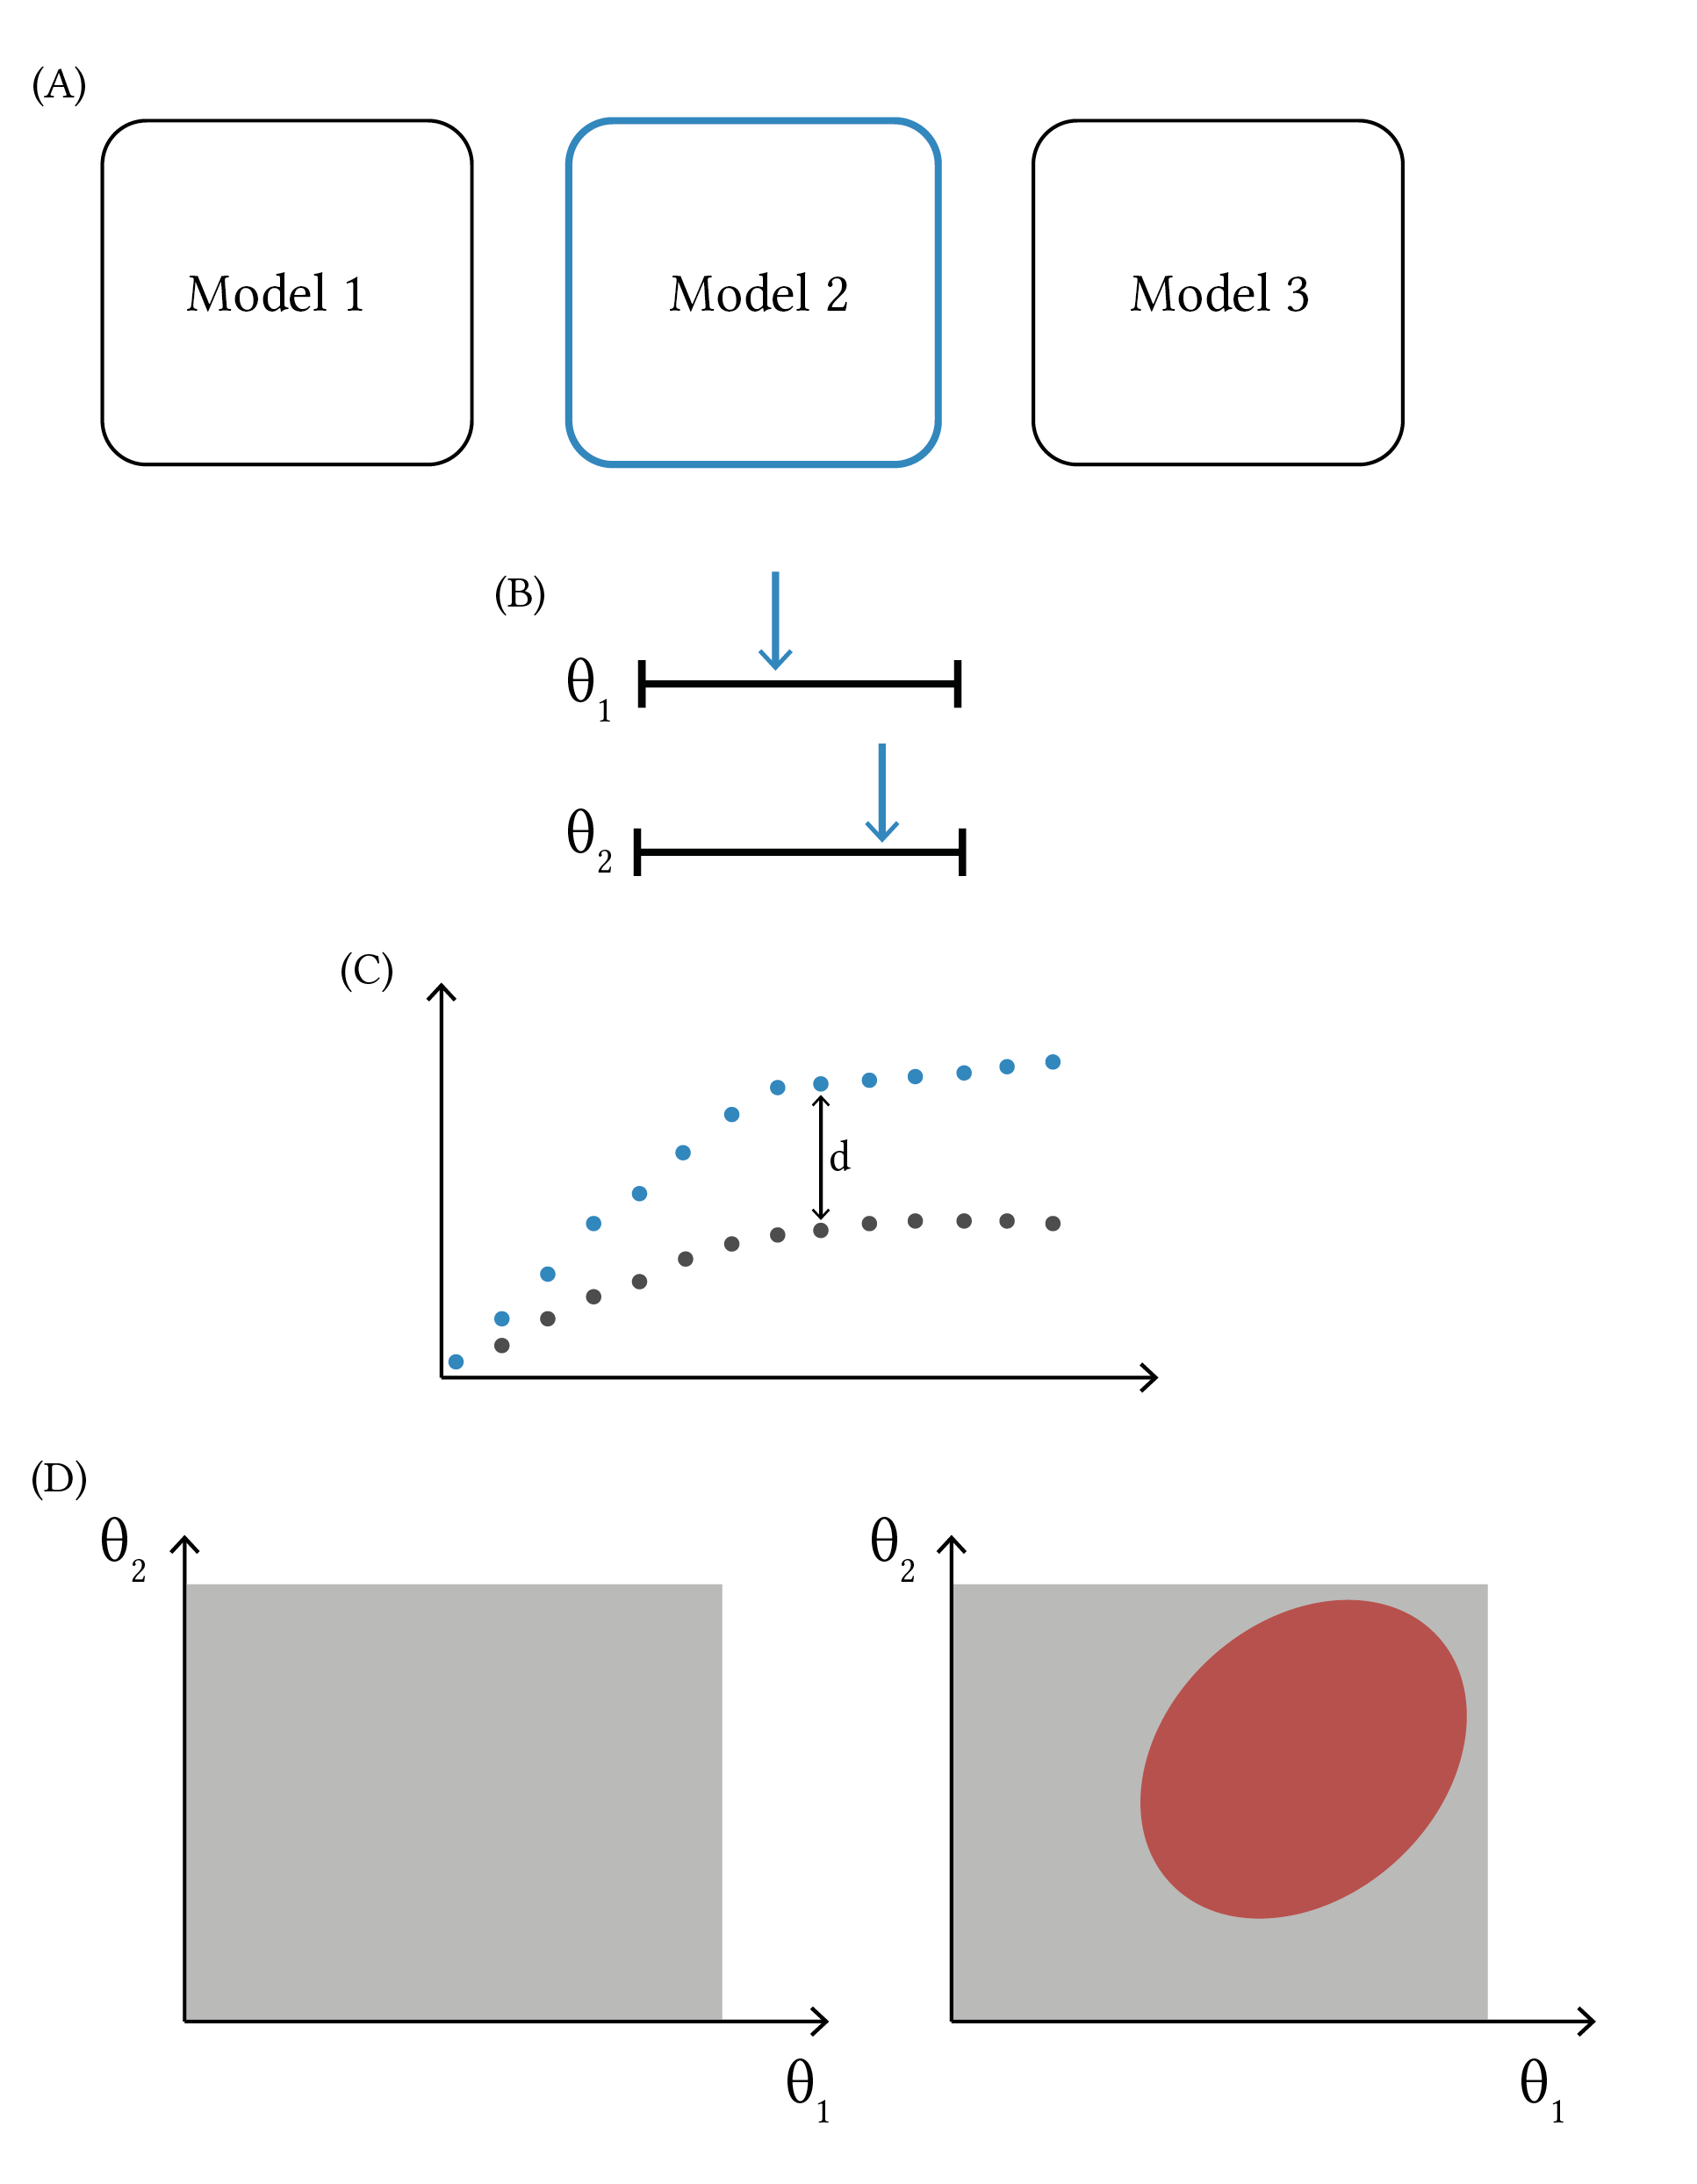
\includegraphics[scale=0.5]{../../chapters/chapterABCSysBio/images/model_selection.png}
\caption[LoF caption]{\label{fig:abc_model_sel}: Model selection}
\end{center}
\end{figure*}
\clearpage


In order to select for the more robust toggle switch, the standard toggle switch will be compared to switches with positive auto-regulation in one or both nodes. The more realistic mass action models were used for model selection, with the addition of two inducers, one turning the switch on by repressing AA and one turning the switch off by repressing BB. The following equations are added to the equations of the simple toggle switch used in Section~\ref{sec:paramscan}. Toggle switches with autoregulation on both nodes have both relevant sets of equations added. 

Positive autoregulation on A:

$$
\begin{array}{cccc} 
    \textrm{A2} + \textrm{gA} \stackrel{\textrm{aut 1}}{\longrightarrow} \textrm{A2gA} \\
    \textrm{A2gA} \stackrel{\textrm{aut 2}}{\longrightarrow} \textrm{A} + \textrm{A2gA}\\
    \textrm{A2gA} \stackrel{\textrm{aut 3}}{\longrightarrow} \textrm{A2}+ \textrm{gA}  \\
\end{array}
$$

Positive autoregulation on B:

$$
\begin{array}{cccc} 
    \textrm{B2} + \textrm{gB} \stackrel{\textrm{aut\_1}}{\longrightarrow} \textrm{B2gB} \\
    \textrm{B2gB} \stackrel{\textrm{aut\_2}}{\longrightarrow} \textrm{B} + \textrm{B2gB}\\
    \textrm{B2gB} \stackrel{\textrm{aut\_3}}{\longrightarrow} \textrm{B2}+ \textrm{gB}  \\
\end{array}
$$

%Negative autoregulation on A:
%
%$$
%\begin{array}{cccc} 
%    \textrm{A2} + \textrm{gA} \stackrel{\textrm{aut\_1}}{\longrightarrow} \textrm{A2gA} \\
%    \textrm{A2gA} \stackrel{\textrm{aut\_2}}{\longrightarrow} \textrm{A2}+ \textrm{gA}  \\
%\end{array}
%$$
%
%Negative autoregulation on B:
%
%$$
%\begin{array}{cccc} 
%    \textrm{B2} + \textrm{gB} \stackrel{\textrm{aut\_1}}{\longrightarrow} \textrm{B2gB} \\
%    \textrm{B2gB} \stackrel{\textrm{aut\_2}}{\longrightarrow} \textrm{B2}+ \textrm{gB}  \\
%\end{array}
%$$

Given the models shown above and the parameter priors used for the standard toggle switch parameter inference, ABC SMC model selection is carried out. The results are shown in Figure~\ref{fig:model_sel_res}. The toggle switch with positive autoregulation on A is found as the most robust model using ABC-SysBio. 



\begin{figure*}[htbp]
	\begin{center}
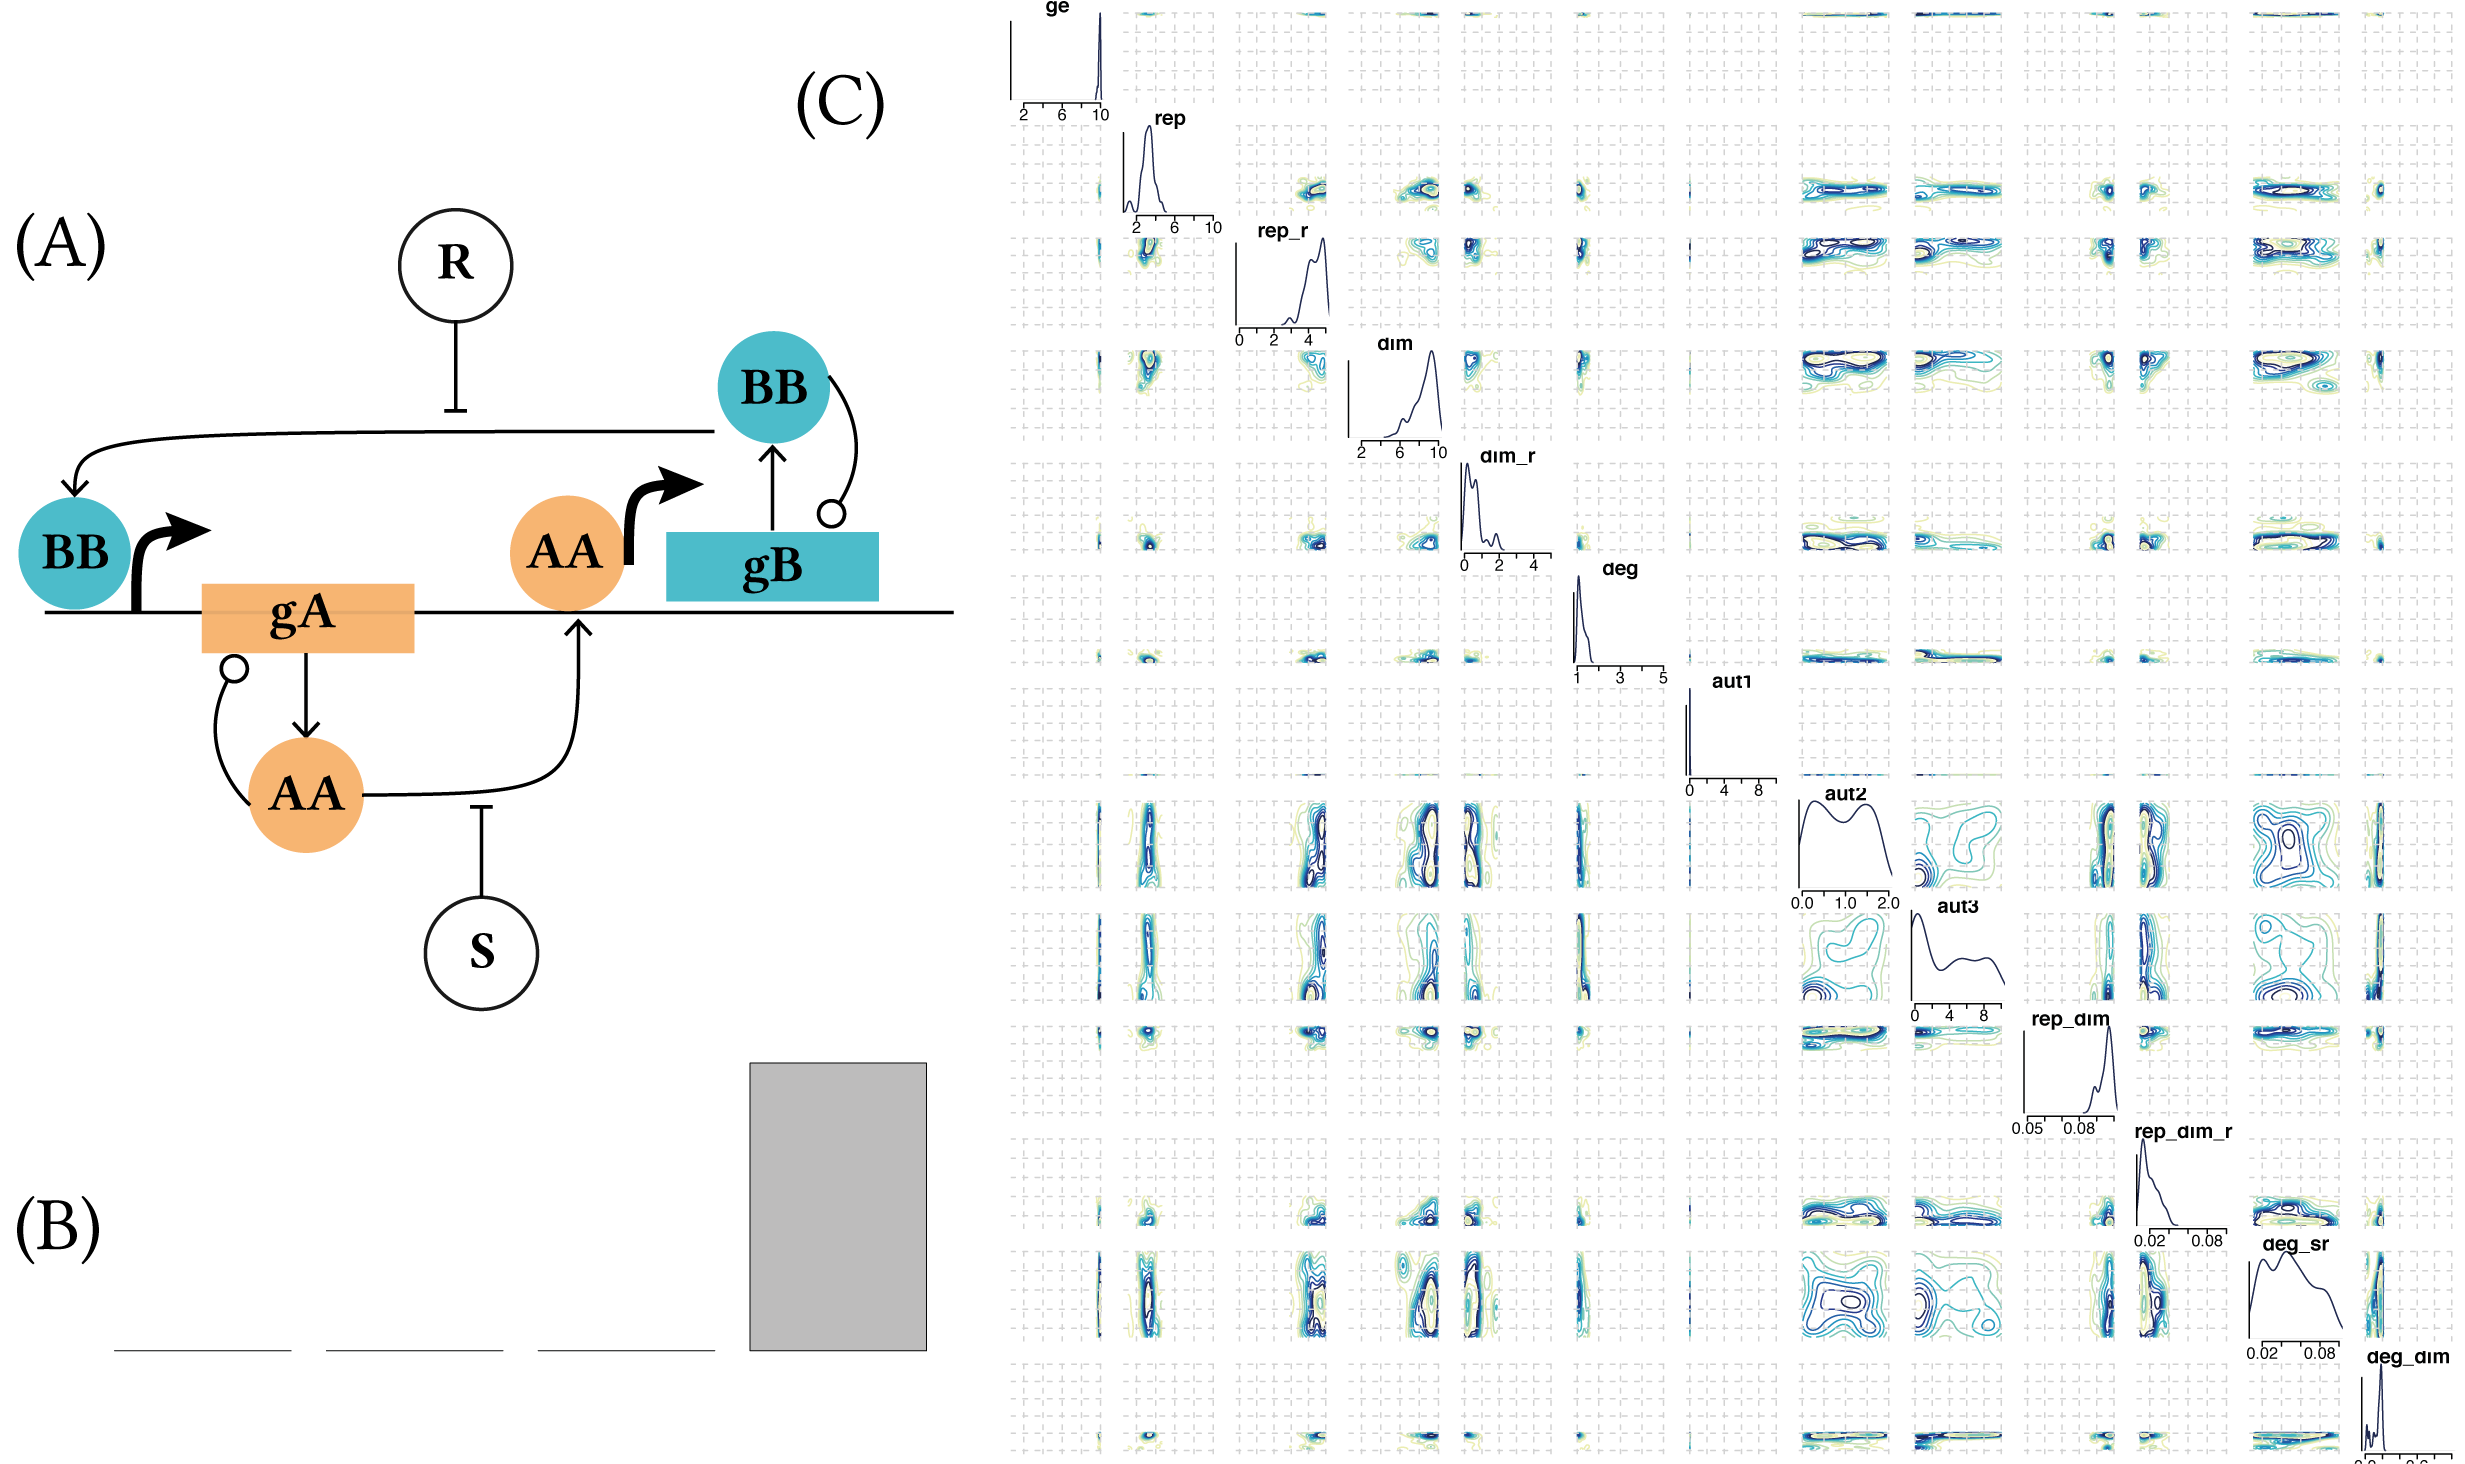
\includegraphics[scale=0.75]{../../chapters/chapterABCSysBio/images/model_sel_res.png}
\caption[LoF caption]{\label{fig:model_sel_res}: (A) The toggle switch models considered. Interactions denoted by a circular arrow head can be positive of zero. (B) The toggle switch with positive autoregulation on A was found to be the most robust to parameter fluctuations. (C) The posterior distribution of the toggle switch with positive autoregulation on A.}
\end{center}
\end{figure*}
\clearpage

\section{Discussion}

Constraints are too many for accurate analysis (the behaviour is too specific).
%From parameter scan
Further analysis is thus needed to determine what these combinations are. A sensitivity analysis of the model will be carried out in order to determine which parameters affect bistability and to which parameters is the system robust. The parameter scan will also be incorporated into the ABC SMC methodology, in order to identify the parameter values required for bistability more efficiently.             

In this work it was shown that a range of stability profiles are achievable by the standard toggle switch. The patterns of the parameter values required for each are beginning to emerge. Further work is required in order to get a definitive answer for the stability characteristics of the toggle switch given this modelling approach.


\clearpage
\section{Summary}

In this chapter I studied the~\textcite{Gardner:2000vha} toggle switch and showed that it is bistable. I further studied the genetic toggle switch by using mass action to represent the model, and removing the \acrshort{qssa} approximation from the models. I identified the parameter ranges that produce a bistable behaviour and could be used as prior distributions for parameter inference. Further, I studied the effect of adding feedback loops has on the robustness of the genetic toggle switch. In the next chapter I address these shortcomings by developing a new algorithm, StabiliyFinder. 


